%%%%%%%%%%%%%%%%%%%%%%%%%%%%%%%%%%%%%%%%%
% Masters/Doctoral Thesis 
% LaTeX Template
% Version 2.5 (27/8/17)
%
% This template was downloaded from:
% http://www.LaTeXTemplates.com
%
% Version 2.x major modifications by:
% Vel (vel@latextemplates.com)
%
% This template is based on a template by:
% Steve Gunn (http://users.ecs.soton.ac.uk/srg/softwaretools/document/templates/)
% Sunil Patel (http://www.sunilpatel.co.uk/thesis-template/)
%
% Template license:
% CC BY-NC-SA 3.0 (http://creativecommons.org/licenses/by-nc-sa/3.0/)
%
%%%%%%%%%%%%%%%%%%%%%%%%%%%%%%%%%%%%%%%%%

%----------------------------------------------------------------------------------------
%	PACKAGES AND OTHER DOCUMENT CONFIGURATIONS
%----------------------------------------------------------------------------------------

\documentclass[
11pt, % The default document font size, options: 10pt, 11pt, 12pt
%oneside, % Two side (alternating margins) for binding by default, uncomment to switch to one side
english, % ngerman for German
singlespacing, % Single line spacing, alternatives: onehalfspacing or doublespacing
%draft, % Uncomment to enable draft mode (no pictures, no links, overfull hboxes indicated)
%nolistspacing, % If the document is onehalfspacing or doublespacing, uncomment this to set spacing in lists to single
%liststotoc, % Uncomment to add the list of figures/tables/etc to the table of contents
%toctotoc, % Uncomment to add the main table of contents to the table of contents
%parskip, % Uncomment to add space between paragraphs
%nohyperref, % Uncomment to not load the hyperref package
headsepline, % Uncomment to get a line under the header
%chapterinoneline, % Uncomment to place the chapter title next to the number on one line
%consistentlayout, % Uncomment to change the layout of the declaration, abstract and acknowledgements pages to match the default layout
]{MastersDoctoralThesis} % The class file specifying the document structure

\usepackage[utf8]{inputenc} % Required for inputting international characters
\usepackage[T1]{fontenc} % Output font encoding for international characters

\usepackage{mathpazo} % Use the Palatino font by default

\usepackage[backend=bibtex,style=numeric,natbib=true]{biblatex} % Use the bibtex backend with the authoryear citation style (which resembles APA)

\addbibresource{multi-authority-abe.bib} % The filename of the bibliography

\usepackage[autostyle=true]{csquotes} % Required to generate language-dependent quotes in the bibliography
\usepackage{makecell}
\renewcommand\theadfont{\bfseries}
\renewcommand\theadalign{bl}
\renewcommand\cellalign{cl}

\usepackage{acro}
\acsetup{first-style=short}
\usepackage{amsmath}
\usepackage[titletoc,toc,title]{appendix}
\usepackage{listings}
\lstset{basicstyle=\ttfamily\scriptsize}


\usepackage[textsize=footnotesize]{todonotes} % for todo notes
% define new command for \req (bold and italic)
\newcommand{\req}[1]{\textbf{\textit{#1}}}

% use \todo[inline] per default
\let\originaltodo\todo
\renewcommand{\todo}{\originaltodo[inline]}

\newcommand{\question}[1]{\originaltodo[color=green, inline]{#1}}


%----------------------------------------------------------------------------------------
%	MARGIN SETTINGS
%----------------------------------------------------------------------------------------

\geometry{
	paper=a4paper, % Change to letterpaper for US letter
	inner=2.5cm, % Inner margin
	outer=3.8cm, % Outer margin
	bindingoffset=.5cm, % Binding offset
	top=1.5cm, % Top margin
	bottom=1.5cm, % Bottom margin
	%showframe, % Uncomment to show how the type block is set on the page
}

%----------------------------------------------------------------------------------------
%	THESIS INFORMATION
%----------------------------------------------------------------------------------------

\thesistitle{Practical Multi-Authority Attribute-Based Encryption for Secure Cloud Storage Systems} % Your thesis title, this is used in the title and abstract, print it elsewhere with \ttitle
\supervisor{Prof. Dr. Florian \textsc{Tschorsch}} % Your supervisor's name, this is used in the title page, print it elsewhere with \supname
\examiner{} % Your examiner's name, this is not currently used anywhere in the template, print it elsewhere with \examname
\degree{Master of Science} % Your degree name, this is used in the title page and abstract, print it elsewhere with \degreename
\author{Marvin \textsc{Petzolt}} % Your name, this is used in the title page and abstract, print it elsewhere with \authorname
\addresses{} % Your address, this is not currently used anywhere in the template, print it elsewhere with \addressname

\subject{Computer Sciences} % Your subject area, this is not currently used anywhere in the template, print it elsewhere with \subjectname
\keywords{} % Keywords for your thesis, this is not currently used anywhere in the template, print it elsewhere with \keywordnames
\university{\href{https://tu-berlin.de}{Technical Unisersity Berlin}} % Your university's name and URL, this is used in the title page and abstract, print it elsewhere with \univname
\department{\href{https://dsi.tu-berlin.de}{Distributed Systems Infrastructure}} % Your department's name and URL, this is used in the title page and abstract, print it elsewhere with \deptname
\group{\href{https://www.eecs.tu-berlin.de/menue/fakultaet_iv/?no_cache=1}{\textsc{Faculty} IV,}} % Your research group's name and URL, this is used in the title page, print it elsewhere with \groupname
\faculty{\href{https://www.eecs.tu-berlin.de/menue/fakultaet_iv/?no_cache=1}{\textsc{Faculty} IV}} % Your faculty's name and URL, this is used in the title page and abstract, print it elsewhere with \facname

\AtBeginDocument{
\hypersetup{pdftitle=\ttitle} % Set the PDF's title to your title
\hypersetup{pdfauthor=\authorname} % Set the PDF's author to your name
\hypersetup{pdfkeywords=\keywordnames} % Set the PDF's keywords to your keywords
}

\DeclareAcronym{AA}{
  short = AA ,
  long  = Attribute Authority ,
  class = abbrev
}

\DeclareAcronym{CA}{
  short = CA ,
  long  = Central Authority ,
  class = abbrev
}

\DeclareAcronym{CSP}{
  short = CSP ,
  long  = Cloud Storage Provider ,
  class = abbrev
}

\DeclareAcronym{ABE}{
  short = ABE ,
  long  = Attribute-Based Encryption ,
  class = abbrev
}

\DeclareAcronym{CP-ABE}{
  short = CP-ABE ,
  long  = Ciphertext policy Attribute-Based Encryption ,
  class = abbrev
}

\DeclareAcronym{KP-ABE}{
  short = CP-ABE ,
  long  = Key policy Attribute-Based Encryption ,
  class = abbrev
}

\DeclareAcronym{HABE}{
  short = HABE ,
  long  = Hirachical Attribute-Based Encryption ,
  class = abbrev
}

\DeclareAcronym{DABE}{
  short = CP-ABE ,
  long  = Decentralized Attribute-Based Encryption ,
  class = abbrev
}

\DeclareAcronym{MA-ABE}{
  short = MA-ABE ,
  long  = Multi-Authority Attribute-Based Encryption ,
  class = abbrev
}

\DeclareAcronym{DAC-MACS}{
  short = DAC-MACS ,
  long  = Effective Data Access Control for Multi-Authority Cloud Storage Systems ,
  class = abbrev
}

\DeclareAcronym{TF-DAC-MACS}{
  short = TF-DAC-MACS ,
  long  = Two-Factor DAC-MACS ,
  class = abbrev
}


\begin{document}

\frontmatter % Use roman page numbering style (i, ii, iii, iv...) for the pre-content pages

\pagestyle{plain} % Default to the plain heading style until the thesis style is called for the body content

%----------------------------------------------------------------------------------------
%	TITLE PAGE
%----------------------------------------------------------------------------------------

\begin{titlepage}
\begin{center}

\vspace*{.06\textheight}
{\scshape\LARGE \univname\par}\vspace{1.5cm} % University name
\textsc{\Large Master Thesis}\\[0.5cm] % Thesis type

\HRule \\[0.4cm] % Horizontal line
{\huge \bfseries \ttitle\par}\vspace{0.4cm} % Thesis title
\HRule \\[1.5cm] % Horizontal line
 
\begin{minipage}[t]{0.4\textwidth}
\begin{flushleft} \large
\emph{Author:}\\
\authorname % Author name - remove the \href bracket to remove the link
\end{flushleft}
\end{minipage}
\begin{minipage}[t]{0.4\textwidth}
\begin{flushright} \large
\emph{Supervisor:} \\
\supname % Supervisor name - remove the \href bracket to remove the link  
\end{flushright}
\end{minipage}\\[3cm]
 
\vfill

\large \textit{A thesis submitted in fulfillment of the requirements\\ for the degree of \degreename}\\[0.3cm] % University requirement text
\textit{in the}\\[0.4cm]
\groupname\\\deptname\\[2cm] % Research group name and department name
 
\vfill

{\large \today}\\[4cm] % Date
%\includegraphics{Logo} % University/department logo - uncomment to place it
 
\vfill
\end{center}
\end{titlepage}

%----------------------------------------------------------------------------------------
%	DECLARATION PAGE
%----------------------------------------------------------------------------------------

\begin{declaration}
\addchaptertocentry{\authorshipname} % Add the declaration to the table of contents
\noindent I, \authorname, declare that this thesis titled, \enquote{\ttitle} and the work presented in it are my own. I confirm that:

\begin{itemize} 
\item This work was done wholly or mainly while in candidature for a research degree at this University.
\item Where any part of this thesis has previously been submitted for a degree or any other qualification at this University or any other institution, this has been clearly stated.
\item Where I have consulted the published work of others, this is always clearly attributed.
\item Where I have quoted from the work of others, the source is always given. With the exception of such quotations, this thesis is entirely my own work.
\item I have acknowledged all main sources of help.
\item Where the thesis is based on work done by myself jointly with others, I have made clear exactly what was done by others and what I have contributed myself.\\
\end{itemize}
 
\noindent Signed:\\
\rule[0.5em]{25em}{0.5pt} % This prints a line for the signature
 
\noindent Date:\\
\rule[0.5em]{25em}{0.5pt} % This prints a line to write the date
\end{declaration}

\cleardoublepage

%----------------------------------------------------------------------------------------
%	QUOTATION PAGE
%----------------------------------------------------------------------------------------

%\vspace*{0.2\textheight}

%\noindent\enquote{\itshape Thanks to my solid academic training, today I can write hundreds of words on virtually any topic without possessing a shred of information, which is how I got a good job in journalism.}\bigbreak

%\hfill Dave Barry

%----------------------------------------------------------------------------------------
%	ABSTRACT PAGE
%----------------------------------------------------------------------------------------

\begin{abstract}
\addchaptertocentry{\abstractname} % Add the abstract to the table of contents
Commonly a group of users want to share a ciphertext, they need to agree on a shared key. In order to ensure forward and backward secrecy, this shared key needs to be updated and distributed to every member everytime a user leaves or joins the group. Classical encryption methods encounter their limits, in which this approach is no longer feasible for a large number of users. In this work the field of attribute based encryption (ABE) have been analyzed to solve this issue for a secure cloud storage environment. Different ABE schemes haven been compared for their applicability in Bdrive. Finally, the implementation of the adapted scheme was evaluated for performance, scalability and security, showing that secure group communication using ABE can achieve sub-linear rekeying overhead. 
\end{abstract}

%----------------------------------------------------------------------------------------
%	ACKNOWLEDGEMENTS
%----------------------------------------------------------------------------------------

% \begin{acknowledgements}
% \addchaptertocentry{\acknowledgementname} % Add the acknowledgements to the table of contents
%The acknowledgments and the people to thank go here, don't forget to include your project advisor\ldots
%\end{acknowledgements}

%----------------------------------------------------------------------------------------
%	LIST OF CONTENTS/FIGURES/TABLES PAGES
%----------------------------------------------------------------------------------------

\tableofcontents % Prints the main table of contents

% \listoffigures % Prints the list of figures

% \listoftables % Prints the list of tables

%----------------------------------------------------------------------------------------
%	ABBREVIATIONS
%----------------------------------------------------------------------------------------

%\begin{abbreviations} % Include a list of abbreviations (a table of two columns)

%\printacronyms

%\end{abbreviations}

%----------------------------------------------------------------------------------------
%	THESIS CONTENT - CHAPTERS
%----------------------------------------------------------------------------------------

\mainmatter % Begin numeric (1,2,3...) page numbering

\pagestyle{thesis} % Return the page headers back to the "thesis" style

% Introduction / Background  / Problem description
\section{Introduction}
\label{sec:introduction}
\todo{
    * **Introduction**\\
    * Ruff problem describtion\\
    * How \ac{ABE} can solve this\\
    * How \ac{ABE} works\\
    * Short history summary of \ac{ABE}\\
    * What is expected of this work\\
    * What are the targets
}
\lettrine[nindent=0em,lines=3]{I}n public-key cryptography each user is identified by his unique public and private key pair. Peer-to-peer communication works well with this scheme, but as soon as an encrypted content needs to be accessed by multiple participants, the data owner has to encrypt the content for each user explicitly. This results in many encrypted versions of the same  file, each secured by a different public key. Such scheme does not scale in the secure cloud storage domain. Here often data holders want to share the same content with many other users at the same time.

We reach the point where the classical public-key end-to-end encryption scheme does not scale anymore. We would like to employ an encryption scheme which has a constant number of access keys regardless of the number of participants.
\todo{extend}

\subsection{Secure cloud storage system}
In the past 20 year we witnessed a shift of resource consumption on the user side to outsourcing more and more resources into the cloud. Naturally, users moved their files and pictures into cloud storage systems. This helped companies to maintain an ecosystem around the user helping him to synchronize his files and photos to different devices.  

With increasing transparency raised also the concern that it was not clear anymore who could access the private files especially when they are transmitted and stored on oversee servers. Bdrive, a secure cloud storage system, promises to not export files and data to other countries. It splits up files in smaller chunks that are saved separately on different cloud storage provider (\ac{CSP}). To ensure end-to-end encryption a Bdrive client encrypts locally each of its chunks with a one-time symmetric key that is then encrypted under its own public key. This encrypted key is called a file key and it is uploaded to the Bdrive server where it is stored securely (see figure \ref{fig:filekey}).

\subsection{Rekeying}
\subsection{Background}
\begin{figure*}[!ht]
\centering
    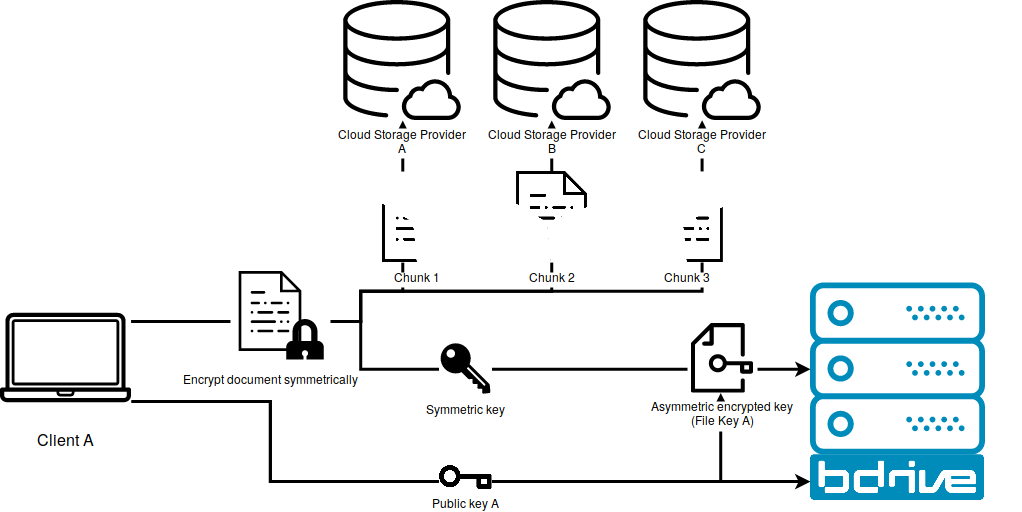
\includegraphics[width=0.8\linewidth]{img/bdrive1.png}\par 
    \caption{Client uploads an encrypted file to the \ac{CSP}s and the file key and public key to Bdrive.}
    \label{fig:filekey}
\end{figure*}
\begin{figure*}[!ht]
\centering
    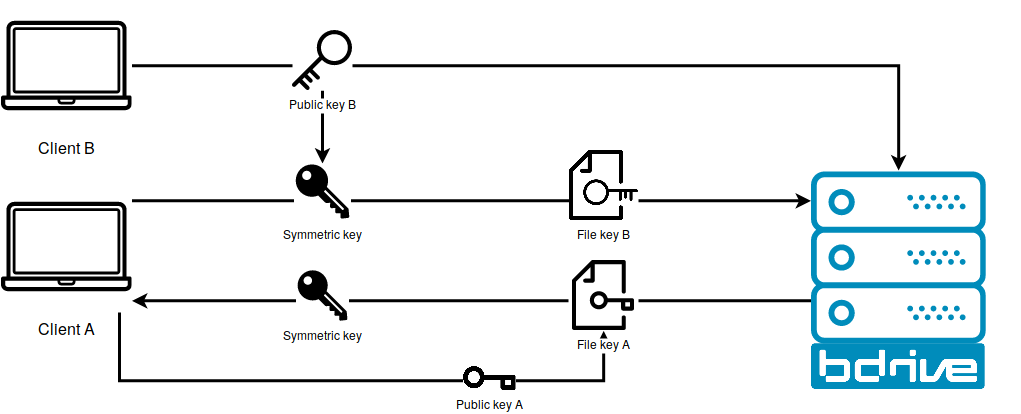
\includegraphics[width=0.8\linewidth]{img/bdrive2.png}\par
    \caption{Client A grants Client B access to the uploaded file by re-keying the file key}
    \label{fig:rekey}
\end{figure*}
Since each device of the same user has a different private-public key pair, the device is in charge of making the file keys accessible for a new device. This will be done by downloading each file key for the respective file, receiving the public key of the new device, decrypting the file key with its own private key, encrypting it again with the public key of the new device and finally, uploading the new file key to the Bdrive server. This process will be called re-keying (see figure \ref{fig:rekey}). In the later sections we will referee to clients as devices. 

% File upload and file key creation
In Bdrive each device of a user generates a new \ac{RSA} key pair on registaion. The fingerprint (hash) of the public key identifies the device uniquly. To save a file in the cloud the device fist encrypes the file symmetrically with the so called "filekey". The filekey equals the hash of the plain file content and so ensures tamperproofness and integrity on decryption. End-to-end encryption implies that the server should never be able to decrypt the file by itself. To enforce this the device encrypts the filekey asymmetrically with its own public key before uploading the filekey to the Bdrive server where it is stored securly. In Bdrive, the encrypted file chunks are uploaded to the different cloud storage provider (\ac{CSP}). 

% Access file
If the user wants to access a file locally, the devices requests the encrypted filekey from the server and downloads the file chunks from the \ac{CSP}s. Locally, it decrypts the filekey with his private key and finally deciphers the assembled file with the decrypted filekey. 

% Process for multibe devices
So far we took a look on how the encryption process is handled for a single device. However, this process turns out to be much more computationally complex in a multiple device setting.  If a user registers more then one device the existing data needs to be synchronized to the new device. The server notifies the existing device for the newly registered one and the public key of the new device is downloaded. Now the existing device needs to download each filekey for each file of the user and decrypts it. The synchronization is finished by encrypting the filekeys with the new devices public key and uploaded again to the server. The new device can now start to download and decrypt the file chunks as described previously.

Usually in cloud storage systems we also have the concept of groups. They are a collection of clients which share data between them. For that they form a so called \textit{share}. To somehow express the overhead of joining or leaving a share we will use the following notation. $f$ and $n$ donate the creation of the number of filekeys and is the number of devices in a share respectively.

% Adventages
If a new devices joins a share in Bdrive we need to make the existing file keys available to the new devices which results in $O(f)$ additional encryptions, messages and keys. However, a big advantage of this scheme is that forward secrecy\footnote{Forward Secrecy: The left entity will have no knowledge about future shared content.} will not produce additional overhead. We simply remove all the filekeys belonging to the left device and do not further encrypt new uploaded files for this device anymore. The backward secrecy constraint, while being an imported security feature, will explicitly be broken by clients. This is due a data owner invites a new member into a group he wishes that the new member receives all previous uploaded content. Bdrive is ensuring this by explicitly reencrypting all file keys for the new device. 

\subsection{Problem description}
% Bdrive rekeying
% Motivation and Problem description

% Disadventages in shares
Notice, that this approach does not scalable for a large number of devices. Lets look at the use case of creating a new share. Each device of invited to a share needs to have an own version of the file key, encrypted with the devices public key, issued. This process scales with $O(n * f)$ keys. 
%Were $n$ donates the number of devices involved in the sharing and $f$ the number of file versions in the share.\footnote{Each file consist of many file versions. Each file version needs an own file key since for each content change a new file is updated.}
Further, we need to send the same number of messages containing the encrypted file key and we need to encrypt each filekey $n$ times which also results in $O(n * f)$ encryptions in total. 

To informally describe this problem lets assume we have an CEO of a 50 employee company who wants to create a company wide share. Each of the employee has at least two devices (say one web view client and a desktop client). To upload the latest presentation the client of the CEO know has to create $50 * 2 = 100$ filekeys to upload, $100$ messages to distribute $100$ encryptions to make. Even worst for each new presentation upload another $100$ filekeys need to be maintained. In a large scale company this overhead becomes unmaintainable.

\subsection{Attribute-Based encryption}
\textit{Attribute-Based Encryption} (\ac{ABE}) defines users over attributes and attribute keys rather then its individual public key. Since users are not unique among their attribute set it is possible to reduce the number of needed keys of a share to the number of attributes necessary to describe the group completely. 

Attributes are issued by a \textit{Attribute Authority} (\ac{AA}). This authority has global decryption power in the domain it administers. For that reason we need to split up the attributes into different domains, each managed by an own AA. In the use case of cloud storage systems for business it makes sense to setup an own AA for each company.

With ABE we also get the advantage of defining access policies for cipher texts. This policies consist of boolean formulas with attribute values as inputs. Only if a user satisfies the given policy he is able to decipher the cipher text.

In our use case inter company sharing becomes tricky. Now different AAs need to cooperate to create cipher text policies containing attributes of the whole ecosystem.  

ABE scales with the number of attributes contained in a cipher text. Usually some could assume that the set of attributes is smaller than the total number of devices in the ecosystem. Which makes ABE scale better then the current rekeying scheme in Bdrive. 

\subsection{Contribution}
The target of this work is to find a more scalable solution to the currently enrolled re-keying scheme in the domain of secure cloud storage systems. Different schemes need to be evaluated against each other to find most scalable solution and with respect to the requirements of section section \ref{sec:requirements}. Further, intra-company management (each company administrates only its own domain) and inter-company file sharing (it is possible to share files across companies) should still be possible. The selected scheme should be practically applicable in the real world.

% Related overview schemes and cloud storage evaluation
 \chapter{Related Work}
\todo{
	Cite \cite{lee2013survey} and similar overview paper
}

In the litrature exist different overview and comparison paper of the different schemes. 

% \subsection{Attribute-Based Encryption}
% Attribute Based Encryption (\ac{ABE}), first introduced by Sahai and Waters \cite{sahai2005fuzzy}, is a cryptographic encryption scheme which uses attributes of a user as keys for encryption. This enables the data owner to craft a ciphertext over chosen attributes that can only be decrypted by any entity that holds a super set of matching attributes. Further, it is possible to embed a complex access structure (e.g. access trees) inside the cipher text, where each node contains \textit{\ac{AND}} or \textit{\ac{OR}} threshold gates. This approach is known as Ciphertext-Policy Attribute-Based Encryption (\ac{CP-ABE}) \cite{bethencourt2007ciphertext}. 
% It is also possible to do it the other way around: Associate the user's key with an access policy, formally known as Key-Policy Attribute Based Encryption (\ac{KP-ABE}) 	te{goyal2006attribute}. 
% %Now the encryptor needs only to encrypt a given plain text with the public key of specific attributes so that only users who hold the right keys are able to decrypt the cipher text.

% Both approaches are limited to one attribute authority (\ac{AA}). So only one trusted entity is in charge of issuing attributes and their matching key pairs. However, in the real world we would like to distribute the issuing of attributes over different authorities. A new scheme is needed where different attribute authorities cooperate and communicate across different domains.  

% % The basic idea is, as proposed in \cite{chase2007multi}, to construct for each users a polynomial of degree $d-1$, where $d$ donates the number of attributes in our system. 

% Multi-Authority Attribute Based Encryption (\ac{MA-ABE}), first proposed by Chase 2007 \cite{chase2007multi}, allows multiple attribute authorities to maintain different attribute domains. To ensure collusion resistance between users, a trusted  Central Authority (\ac{CA}) was introduced to assign each user an unique identifier (\ac{UID}) and making the decryption process depending on this \ac{UID}. Its disadvantage is the \ac{CA}'s global decryption power and therefore the necessity to remain trusted. 
% %To prevent collusion between user in a multi authority setting, the challenge for each user needs to be individual. But it still needs to be ensured that the encryption of a message is independent of any user specific identifier, since the encryption progress should sourly depend on the attribute set known to the system.
% %To mitigate this problem a global identifier (\ac{GID} or \ac{UID}) per users was introduced that is shown to each attribute authority (\ac{AA}) to receive the corresponding private key for the users attributes. 
% %The central authority (\ac{CA}) now has to make sure that the user dependent challenge results in a global decryption key to decrypt the message.
% %In fact the \ac{CA} has to be trusted since it computes the users private keys in such a way that on decryption it reveals the global decryption key. 
% Chase \textit{et al.} addressed this issue in \cite{chase2009improving} by distributing the global secret  master key generation over the \ac{AA}s. However, since the global master secret is computed on system initialization, no further \ac{AA}s can be added afterwards without rebooting the system. Also the scheme did not support attribute revocation which rendered it practical not applicable.
% % Each authority uses this seed in combination with a pseudo random function to deterministically create the users private key. Since the \ac{CA} possesses the same seed, same pseudo random function and issues the users \ac{GID}, it can also compute the same private key as issued by the corresponding \ac{AA}. So it can ensure that on decryption the keys add up to reveal the global decryption key. This scheme has a major issue: The \ac{CA} has global decryption power. 

% % Chase notices this problem as well and tried to mitigate it by decentrializing the seed generation \cite{chase2009improving}.  First user attributes could not easly be revoked\footnote{Chase proposed to assign each user a range of \ac{GID}s, so that a user can migrate to the next \ac{GID} on revocation. Since the \ac{GID} range is finite, this solution does not scale.}. Second \ac{AA}'s cant be added on runtime without reissuing each user his keys. And last, the attribute universe is finite (no large-universe). Further we noticed that if a failure of one \ac{AA} renders the system unresponsible, since a cyphertext includes attributes from each authority. 

% Data Access Control for Multi-Authority Cloud Storage Systems (\ac{DAC-MACS}) \cite{yang2013dac} is a scheme that tackles both of this issues. Each authority receives its own ciphertext that depends solely on the attributes issued in this domain. While Chase managed to maintain the "one-plaintext-one-ciphertext" ratio, \ac{DAC-MACS} needs to create $k$ ciphertexts: One per \ac{AA}.\footnote{If the ciphertext does not require any attributes of an specific authority it does not have to create a ciphertext for this domain.} It does not require any coordination between authorities which enables to add new \ac{AA}s at runtime without recreating the user keys. This scheme also includes features for efficient revocation while it claims to maintain forward and backward secrecy. 

% \ac{DAC-MACS} is not collusion resistance on attribute revocation under the active attack model. The scheme \ac{NEDAC-MACS} (New Extended \ac{DAC-MACS}) shows and solves this vulnerability \cite{wu2017security}. Recent studies introduce a more efficient, scalable and secure approaches such as \ac{MAACS} \cite{li2016secure} and \ac{TF-DAC-MACS} (Two-Factor \ac{DAC-MACS} 	te{li2017two}. The \ac{DAC-MACS} family is further known for the proxy decryption technique, first introduced by \cite{li2013matrix}, where a honest-but-curious server helps the user on decryption.

% Priscilla and Nagarajan 2018 \cite{nagarajan2018overview} conducted an analysis of the \ac{DAC-MACS} family. In addition to that work, this thesis will focus on alternative approaches to improve scalability of secure cloud storage systems and analyze the field of \ac{ABE} and \ac{MA-ABE} more deeply.

% Requirements
\section{Requirements}
\label{sec:requirements}
\todo{Take social requirementes into account?}
The general (\textbf{\textit{B*}}) requirements of this thesis will be summarized by two major points: 

\begin{itemize}
	\item[\textit{\textbf{B1}}] \textbf{Performance:} Participating in the system should be possible with low-performance devices (such as smartphones). The overhead for the server on proxy decryption, attribute issuing and revocation should be reasonably low.  
	\item[\textit{\textbf{B2}}] \textbf{Scalability:} The system should scale better than the current encryption scheme with respect to the number of file keys. 
\end{itemize}

In addition, the core (\textbf{\textit{C*}}) security requirements in the context of an \ac{MA-ABE} scheme are the following:
\begin{itemize}
\item[\textit{\textbf{C1}}] \textbf{Collusion resistance:} For two users it should not be possible to combine their attributes to archieve a higher level of decryption power.
\item[\textit{\textbf{C2}}] \textbf{Inter-Company Sharing:} Each company is only responsible for its own domain. This includes attribute and user administration, which translates to secret key generation and revocation. %Since Bdrive would need to consider a multi-authority \ac{ABE} scheme, it should not be possible for a company to decrypt or issue files of other companies if no explicit exception is given for certain files by a trusted company relationship. A companies attribute authority (\ac{AA}) should be responsible for its domain. In the case of an inter company relationship, attributes needs to be issued across different companies. 
\item[\textit{\textbf{C3}}] \textbf{Central Authority:} The \ac{CA} shall not have global decryption power. At most an \ac{AA} can decrypt user files of its own domain.  
\item[\textit{\textbf{C4}}] \textbf{Secret Master key (if any):} Key recovery requires a secret and securely stored master key. It should solely function in the company domain and not globally. 
\item[\textit{\textbf{C5}}] \textbf{Large Attribute and Key Universe:} The number of attributes and users shall not be restricted.
\item[\textit{\textbf{C6}}] \textbf{Adding new Attribute Authorities:} It should be possible to add new attribute authorities at runtime. Without either shutting down the system or recreating each key.
\item[\textit{\textbf{C7}}] \textbf{Untrusted Attribute Authority:} A corrupt Attribute Authority can only harm its own domain, but can not harm the outside system in any way. It cannot gain any additional information.
\item[\textit{\textbf{C8}}] \textbf{Key and Attribute revocation:} Revocation is needed to handle user management in terms of attribute promotion, attribute demotion and key revocation. Forward secrecy should be provided. 
\end{itemize}

\noindent Other (optional \textbf{\textit{O*}}) requirements are: 
\begin{itemize}
	\item[\textit{\textbf{O1}}] \textbf{Traitor tracing:} A user in \ac{ABE} is described by his attribute set and is anonymous in this set. Misbehaving users, who sell their attribute keys to create a decryption black box, should be identifyable. \cite{liu2016practical}
	\item[\textit{\textbf{O2}}] \textbf{Fine-grained access control:} The user shall not be bounded on defining fine-grained access policies which requires either an access tree \cite{bethencourt2007ciphertext} or an linear secret sharing scheme (\ac{LSSS}) \cite{yang2013dac} \cite{li2016secure} \cite{wu2017security} \cite{li2013matrix} \cite{liu2016practical}.
	%Some schemes restrict the user to threshhold access policies, where an user needs at least $n$ of $m$ attributes to encrypt the cipher text. \cite{chase2007multi} \cite{chase2009improving} Other approaches are restriced to $\ac{AND}$ gates which would translate to $m$ of $m$ threshhold gates. \cite{li2017two}
\end{itemize}

% Concept
\chapter{Concept}

% Secure group communication
\section{Secure Group Communication}
The most sophisticated approach to the scalability problem is to create a secret \textit{group key} (\ac{GK}) each time multiple devices need to access the same file. This schemes are called "Secure Group Communication" (\ac{SGC}). The main idea is to reduce the number of filekeys by encrypting all files with a unique \ac{GK} that is only known to the members in the share. Simple approaches use a socalled \textit{Key Distribution Center} (\ac{KDC}) to distribute the group keys to each member. However, while Bdrive could manage forward secrecy quite easily, this schemes suffer from additional reencryption overhead if a member leaves the group. 

% Mutlicast in group communications
Commonoly Secure Group Communications are mentioned together with \textit{multicast messages}. With multicast the same message is distributed to different devices in one setting. In contrast stands \textit{unicast}. Here a central authority is required that manages authentication and authorization to decide which entity should access which content. With multicast messages, however, content is distributed to each entity regardless if this entity is authorized to access this content. Instead authorization is handled via encryption of the content. If an entity owns the key to decrypt the data it is implicitly authorized to access the content as well. Multicast messages are especially handy in group communications since they only need to send one message to distribute the information to all members. As a the trade-off the message size increases.

% The role of \ac{PKI} in group communications
While there are many approaches researching secure group communication and making the rekeying process more efficient, the number of schemes can be reduced to those applicable to secure cloud storage. Here some prerequisites are given that are not generally assumed. Secure cloud storage system often deploy a public key infrastructure (\ac{PKI}) to bind identities to public keys of clients which means that a key exchange already happened.

In contrast to that are schemes that extend the 2-parties Diffie-Hellman (\ac{DH}) key exchange to n-party scheme, such as in \textit{Steiner at. al., 1996} \cite{steiner1996diffie}. The \ac{DH} key exchange is designed for unsecured environments to create a unique communication key, known to every member in the group, but not known to a passive attacker. However, since all communication is already disclosed and secured by the \ac{PKI} those schemes can be eliminated. They suffer from additional computation or message exchange overhead compared to schemes that assume an existing \ac{PKI}.   

In the following it is widely assumed that a client is identified uniquely by its public key, which is also known by the cloud server and can be queried by other clients. 

\subsection{Group Key Management Protocol}
The Group Key Management Protocol (\ac{GKMP}) \cite{harney1997group} addresses the rekeying problem in a simple but scalable way. If a device wants to share files with a group of other clients it creates the group key and encrypts all filekeys with this group key. This \ac{GK} needs to be securely distributed to all members which means that the data owner needs to download and store every public key of the group members and encrypt the \ac{GK} for each of them. Further, the data owner needs to encrypt all shared filekeys symmetrically with the chosen group key. 

% Disadventage
To ensure forward secrecy, the \ac{GK} needs to be renewed every time a member leaves the group. This overhead is located in the same computational magnitude as bootstrapping a new group. 

% Adventage
The big advantage of this scheme, compared to the scheme employed in Bdrive, is that it reduces the overhead of the number of encryptions, messages and keys on new file upload dramatically. While the data owner had to create a filekey for each member respectively, \ac{GKMP} reduces this to one filekey per upload. Additionally, since no backward secrecy have to be ensured, the \ac{GK} only have to be distributed to the new member\footnote{With backward secrecy the GK would have been renewed each time a new member joins.}.

\subsection{Logical Key Hierarchy}
\begin{figure*}[!ht]
\centering
    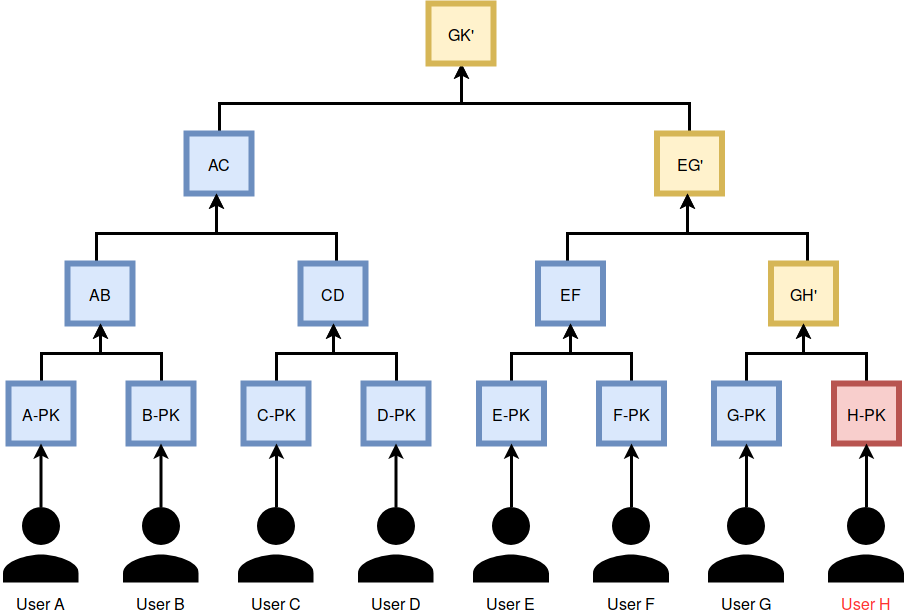
\includegraphics[width=0.8\linewidth]{img/LKH.png}
    \caption{Balanced binary \ac{LKH} and user H leaves the group. Node marked in red is removed from the group. Node marked in yellow require an update and need to be stored locally by any leaf of this node. }
    \label{fig:lkh}
\end{figure*}

Logical Key Hierarchy (\ac{LKH} 	te{wallner1999key} is a \ac{GKMP} that reduces user side storage and rekey transmissions by organizing users keys in a tree hierarchy and maximizing the use of multicast messages. The tree is maintained by a central \textit{Key Distribution Center} (\ac{KDC}). In the work of Wallner \textit{et. al.} \cite{wallner1999key} it is explicitly stated that such trees neither have to be balanced nor binary, but for the sake of simplicity exactly this is assumed. Users (and their respective public keys) are organized at the leafs of the LKH. Each node is composed of a key that is encrypted with its children keys. An encrypted key is known to all leafs related to this node and can, on change of this node, be transmitted in one multicast transmission to all its leafs. The root node summarizes the \ac{GK}. The \ac{GK} is used in the same way as in \ac{GKMP} to secure the group communication. 

While in \ac{GKMP} each user needs to store each members public key to eventually rekey the GK, in \ac{LKH} each user only needs to store $log(n) +1$ keys (path from leaf to root node). Beginning from the bottom, each leaf node could decrypt the next parent node until it arrives at the root node. One other advantage is that many members share the same keys. So it is more efficient to transmit this keys in a multicast setting. \ac{LKH} needs to do $2 log(n)$ multicast transmissions and analogous $2 log(n)$ encryptions on each member leave or join.  Here each updated key in the path from leaf to root node needs to be updated and encrypted two times: One time with the key of right children node and second with the key of the left children node. 

In Figure \ref{fig:lkh} user H recently left the group which means, that to ensure forward secrecy, the keys in node $GH$, $EG$ and $GK$ must be updated. The key server will choose a new $GH'$, $EG'$ and $GK'$, encrypts and distributes them in a bottom up fashion starting by $GH'$. $GH'$ is encrypted with user Gs and user Hs public key (G-PK, H-PK) and transmitted to them respective. Next, user E and F receive in a multicast transmission $EG'$, which is encrypted with $EF$ and user G and H receive in a multicast transmission $EG'$ which is now encrypted with the newly established $GH'$ key. Finally, the GK needs to be updated. For the left sub tree $GK'$ is encrypted with $AC$ and transmitted using multicast to the users A, B, C and D. And for the right sub tree $GK'$ is encrypted with $EG'$ to transmitted using multicast to user E, F, G and H. Adding a user to the group follows the same principle. Backward secrecy is implicitly given and not easily removable from this scheme.

\subsection{One-Way Function Trees}
To reduce the transmission and encryption overhead of $2 log(n)$ even further to $log(n)$ other schemes use pseudorandom functions \cite{canetti1999multicast} or one-way functions \cite{sherman2003key} to compute the required keys in the path. This schemes are strongly related to \textit{Merkle Trees}, since each update of the user set will force an update of the root node: The group key.

Each user stores a blinded key for each sibling node in the path to the root node. Starting from his individual key, a user can compute the blinded version of his key. To compute the next parent key, a user utilizes his blinded key, together with the siblings blinded key, which is fed into a one way function to create the key for the parent node. This node needs to be blinded to serve as the input for the next level. In such way the user can compute the needed keys up to the GK. 

Lets assume the same tree layout as in Figure \ref{fig:lkh} but assume that user H joined the group. Given a cryptographically secure hash function $h$. First, user H needs to receive the blinded keys, $h(AC)$, $h(EF)$ and $h(G-PK)$ which he stores locally in addition to his own public key $H-PK$. \textit{One-Way Function Trees} (\ac{OWFT}) have the same storage overhead as LKH with $log(n) + 1$.  As already known from LKH, $GH$, $EG$ and $GK$ need to updated. This nodes are computed from their children blinded values using a merging function $m$ which takes two inputs and produces one output. This could for example be the concatenation of both inputs and then applying $h$ to receive a fixed length output value. Starting from the bottom,  $GH'$ is computed as $m(h(G-PK), h(G-PK))$, analogous $EG' = m(h(EF), h(GH'))$ and finally the updated group key $GK' = m(h(AG), h(EG')$. The new blinded keys are distributed to their respective users using one multicast transmission each, reducing the transmission and encryption overhead to $log(n)$. If user H leaves the group, user G must come up with a new random secret that he hashes as placeholder for the previous blinded key of H to compute $GH'$. Thus forward and backward secrecy is enforced.


\subsection{Comparison}  

\begin{table*}[!ht]
\centering
\begin{tabular}{l 		| l 						| l 							| l 						| l 						}
 						& \textbf{Bdrive} & \textbf{\ac{GKMP}} \cite{harney1997group} & \textbf{\ac{LKH}} \cite{wallner1999key} & \textbf{\ac{OWFT}} \cite{sherman2003key} \\%\textbf{\ac{GDH}.1 	te{steiner1996diffie}\\
\hline
\textbf{initial share} 																																		\\
keys 					& $nf$	 					& $1$  							& $n-1$  					& $n$	 					\\%& $1$ 			\\
messages (unicast)		& $nf$	  					& $n$ 							& $n(log_2(n) + 1)$ 		& $2n(log_2(n) + 1)$		\\%& $2(n - 1)$	\\
messages (multicast) 	& $nf$	 					& $n$ 							& $log_2(n) + 1$ 			& $n - 2$ 					\\%& $2(n - 1)$ 	\\
encryptions				& $nf$	 					& $f + n$ 						& $f + n -1$				& $f + n -1$				\\%& $f + n$		\\
\hline
\textbf{member join} 																																		\\
keys 					& $f$   					& $1$  							& $3 log_2(n)$				& $log_2(n)$				\\ %& $1$			\\
messages (unicast)		& $f$  						& $1$			 				& $2(n - 1)$				& $n$  						\\ %& $2(n - 1)$	\\
messages (multicast) 	& $f$ 	 					& $1$ 		 					& $2 log_2(n)$				& $log_2(n)$				\\ %& $2(n - 1)$	\\
encryptions				& $f$  						& $f + 1$		 				& $f + 2(log_2(n))$ 		& $f + log_2(n)$			\\ %& $f + 2$	 	\\
\hline
\textbf{member leave}																																		\\
keys 					& $0$						& $1$			  				& $3 log_2(n)$				& $log_2(n)$				\\ %& $1$			\\
messages (unicast)		& $0$						& $n$			 				& $2(n - 1)$ 				& $0$	  					\\ %& $2(n-1)$		\\
messages (multicast)	& $0$						& $n$			 				& $2 log_2(n)$				& $log_2(n)$				\\ %& $2(n-1)$		\\ 
encryptions 			& $0$						& $f + n$ 						& $f + 2 (log_2(n))$ 		& $f + log_2(n)$	 		\\ %& $f+n$			\\
\hline	
\textbf{addition of filekey}																																\\
keys 					& $n$		 				& $0$							& $0$	 					& $0$		 				\\ %& $0$			\\
messages (unicast)		& $n$		 				& $0$	 						& $0$ 						& $0$		 				\\ %& $0$			\\
messages (multicast)	& $n$ 						& $0$ 							& $0$ 						& $0$	 					\\ %& $0$			\\
encryptions				& $n$ 						& $1$ 							& $1$ 						& $1$		 				\\ %& $1$			\\
\hline
\end{tabular}
\caption{Comparison of secure group communication schemes. $n$ donates the number of clients and $f$ the number of file keys. Forward secrecy is ensured in each scheme. Assuming a balanced binary tree as in Figure \ref{fig:lkh}}
\label{tab:comparisons}
\end{table*}

Table \ref{tab:comparisons} will compare the discussed schemes against each other regarding number of keys, messages, and encryptions on initialization of the group, when a member joins or leaves and on addition of a new file. 

It is assumed that clients already downloaded the public keys of their group members. Forward secrecy need to be ensured every time a member leaves the group.
Further, messages in table \ref{tab:comparisons} are transmissions that contain a key. There are also meta messages that notify the members about a new file upload or the removal of a member, etc.  They are ignored since they add a constant overhead to all schemes.  If a message could be processed by multiple communication partners it can be transmitted in multicast transmission. In general it is assumped that $f > n$ holds true, since there are usually more files in a share than devices.

Reviewing the performance comparison, Bdrives scheme is not optimal compared to the different approaches. In fact Bdrive has the worst performance on initialization, addition of a filekey and on average also on member join. However, Bdrive has great performance on member leave since client simply do not have to encrypt anymore for the left member.

Each of the schemes have their own strength and weaknesses. \ac{GKMP} has the smallest initialization overhead and \ac{OWFT} the best rekeying overhead. As some could clearly extract from the table that all secure group communication schemes perform better than Bdrive on file upload. Bdrive needs to distribute and encrypt a new filekey $n$ times for each device while any scheme using a \ac{GK} only needs one encryption and one multi cast transmission. 

Under the assumption that a secure cloud storage does not need backward secret, \ac{GKMP} is selected as most suitable candidate. It has great initialization overhead is easily understandable and profits from the fact that no backward secrecy on member join is needed. \ac{LKH} and \ac{OWFT} both have backward secrecy fixed implemented resulting in a bit more worse performance. 

% intro ABE
\section{An Introduction To The Field Of Attribute-Based Encryption}
A key requirement in security of distributed systems is authenticity. It describes the principle of associating individuals with their digital representation. A so called \textit{public key infrastructure} (\ac{PKI}) uses certificates which validate the public key bound to an identity.

\textit{Identity-Based Encryption} (\ac{IBE}) tries to circumvent this standard by binding identities to unique strings already associated with this identity, such as an email address. If encrypted directly with this identifier, no certificate validation check needs to be done to validate the identity of the recipient. 

\subsection{Identity-Based Encryption}
The idea of using universal identifier instead of public keys to identify individuals goes back until 1984. Shamir proposed the first identity-based encryption scheme\cite{shamir1984identity} which uses a central authority to create for each newly registered user a unique universal identifier (e.g. the email address). This identifier can be used for encryption in the same way as public keys were used. However, the difference to \ac{RSA} is that, since the universal identity is the public key, the use of a certificate to bind the public key to an identity becomes nugatory. 
Since the sender has to know the email address of the recipient anyways he can derivative public key component from it, encrypt the email with this key and can be sure that only the identity owning this email can decipher the content. 

Since this scheme could neither be shown to be practical applicable, nor to proven secure, it was not until 2001 when Boneh and Franklin proposed in \cite{boneh2001identity} a new approach to identity-based encryption. The use of the \textit{Weil pairing} revolutionized the field of identity-based encryption.\footnote{Curious reader can readup on the weil pairing here \cite{Miller2004} \cite{galbraith2008pairings} or here \url{https://medium.com/@VitalikButerin/exploring-elliptic-curve-pairings-c73c1864e627}}

\subsection{Bilinear Mappings}
\label{sec:bilinearmappings}
Bilinear mappings are a tool for \textit{cryptographic pairings} and define the relationship between two cyclic groups of the same order into a third one. A cyclic group $G$ is defined by an generator $g$ of that form that each $g^n \in G$ with $n \in \mathbb{Z}$ completely describes each element in the group $G$.

A bilinear map function $e$, also called \textit{pairing} is now defined as the mapping between two groups of the same order $G_1$ and $G_2$ into $G_t$:

\begin{gather*}
 e : G_1 \times G_2 \rightarrow G_t \\
\text{ such that for all } g_1 \in G_1, g_2 \in G_2, a, b \in \mathbb{Z} \\
e(g_1^a, g_2^b) = e(g_1, g_2)^{ab} 
\end{gather*}

If $G_1$ and $G_2$ describe the same group the mapping is called symmetric. In fact the \textit{decisional bilinear Diffie-Hellman problem} becomes easily computable using bilinear mappings. \cite{bethencourt2015intro}

This construct of pairings is used by many schemes to either distribute a secret or computing the secret without revealing it.

\subsection{Attribute-Based Encryption}
\textit{Attribute-Based Encryption} (\ac{ABE}) is ancestor of IBE. Instead assigning each user a unique identifier, the work of Sahai and Waters \cite{sahai2005fuzzy} describes the approach of assigning each user a descriptive set of attributes. A deeper dig into this topic reveales the well known setup from \ac{IBE}: a central \textit{attribute authority} (\ac{AA}) issues attributes on user registration, binds them to key pairs and serves as a central public-key directory. 

One advantage is that the \ac{AA} doesn't have to be online all the time. Once the attributes are issued and distributed the data owner, without any further interactions with the \ac{AA}, can use those to share content to authorized members. Further, no authorization checks are needed. This follows due to the fact that if the entity was authorized to download the content, it will certainly also be able to decrypt it. 

As already known, content is encrypted using a set of attributes, rather then public keys of individuals. This implies that the data owner encrypting the file does not really know which individual deciphers the ciphertext. Using boolean formula and the given attribute universe, the data owner creates an access policy securing his ciphertext. Any entity owning a certain set of attributes that fulfill this policy is allowed to access the data. This feature comes in handy in specific domains such as the medical domain. Here any set of doctors satisfying certain attribute are able to access the medial record. The patient, as the data owner, does not care about the real identities of the doctors only if they satisfy a specific qualification goal. The same is applicable on file-sharing in the business domain. Here users often share content to roles or group of members and if an employee gets promoted he automatically gets access to the content addressed to his job level. 

Further, user management systems always need a procedure to revoke users and their attributes. 
In general two steps need to be made to revoke an attribute from an user. All users, except the revoked user, need to receive a new private key for this attribute and in addition, each ciphertext encrypted under this revoked attribute need to be updated to ensure forward secrecy. 

In summary ABE provides a big advance for the rekeying problem: Since new members joining a group just receive the respective attribute keys no group key needs to be distributed. Users are automatically member of a group if they satisfy the access policy. With \ac{ABE} it is possible to go beyond the natural limitation of Secure Group Communication schemes which had a lower bound of one key per newly joined member.  

\subsection{Comparing Secure Group Communication To Attribute-Based Encryption}
Comparing \ac{SGC} to \ac{ABE} is non trivial. This is due to a different encryption technique used by \ac{ABE} namely paring. Pairing scales more or less with the overhead of \ac{RSA} rather then \ac{ECC} or block ciphers as stated by \textit{Galbraith et. al.} \cite{galbraith2008pairings}. But to achieve the same bit security, computations in pairing need to happen in a much bigger bit-field and thous rendering \ac{ABE} less performant in comparison to \ac{RSA}. But in specific scenarios \ac{ABE} uses less keys to setup the group communication. In the following thous scenarios will be described and analyzed to find out where this schemes differ and what use-cases \ac{ABE} schemes address.

In a \ac{RSA} sharing scheme, each user has his own public key which needs to be transmitted to a third party to establish a secret connection. Creating a group under this scheme will implicitly force the data owner to retrieve all $n$ public keys of all $n$ group members. The central server needs to provide a \ac{PKI} together with the public keys of each registered user to proof their identity. Thus follows the constrain that the central server needs to be available all the time to provide public keys for new registered users. Each member in the group receives an encrypted copy of the group key. The number of keys in \ac{SGC} scales at least linearly with the number of members. 

\ac{ABE} breaks the constrain that the central server has to be available at all time. This is done by using attribute keys on encryption rather then the users public keys. This reduces the number of keys that need to be maintained to the size of the attribute set describing the group. If an new user is registered in the system no new keys need to be downloaded from the view of the data owner. The registered users retrieves his attribute set and eventually can decrypt the shared files if his attributes satisfy the access policy of the group. Further notable is that the number of keys that are maintained in the group remains constant in $a$. With $a$ donating the number attributes used to describe the group. 

Given this observation it can be stated that \ac{ABE} is adventitious in scenarios where users address an unknown group of individuals. This can be some departments (e.g. attribute: police department of New York), colloquiums (e.g. attribute: chairman of TU-Berlin), or general user groups (attribute issued to all employees working in the security research team).

To better clarify the scalability advantage of \ac{ABE}, GKMP is compared to ABE \footnote{Specifically the ciphertext-policy ABE scheme of \cite{bethencourt2007ciphertext} is used in the comparison.} to evaluate the performance of both encryption schemes in general.

\begin{table*}[!ht]
\centering
\begin{tabular}{l 		| l 						| l 						| l }
 						& \textbf{Bdrive}			& \textbf{\ac{GKMP}} 			& \textbf{\ac{ABE}} 		\\
\hline
\textbf{initial share} 																				\\
keys 					& $O(nf)$ 					& $O(1)$	 				& $O(1)$			\\
messages (unicast)		& $O(nf)$  					& $O(n)$					& $O(n)$			\\
messages (multicast) 	& $O(nf)$ 					& $O(n)$ 					& $O(1)$			\\
encryptions				& $O(nf)$ 					& $O(f + n)$				& $O(a)$ 			\\
\hline
\textbf{member join} 																				\\
keys 					& $O(f)$   					& $O(1)$					& $O(1)$			\\
messages (unicast)		& $O(f)$  					& $O(1)$  					& $O(1)$ 			\\
messages (multicast) 	& $O(f)$ 	 				& $O(1)$					& $O(1)$ 			\\
encryptions				& $O(f)$  					& $O(1)$					& $O(1)$ 			\\
\hline
\textbf{member leave}																				\\
keys 					& $O(0)$					& $O(1)$					& $O(1)$			\\
messages (unicast)		& $O(0)$					& $O(n)$  					& $O(N(a^{-1}))$	\\
messages (multicast)	& $O(0)$					& $O(n)$					& $O(1)$ 			\\ 
encryptions 			& $O(0)$					& $O(f + n)$ 				& $O(F(a^{-1}))$	\\
\hline	
\textbf{addition of filekey}																		\\
keys 					& $O(n)$	 				& $O(0)$					& $O(0)$			\\
messages (unicast)		& $O(n)$	 				& $O(0)$					& $O(0)$			\\
messages (multicast)	& $O(n)$ 					& $O(0)$ 					& $O(0)$			\\
encryptions				& $O(n)$ 					& $O(1)$					& $O(1)$			\\
\hline
\end{tabular}
\caption{Comparison of Bdrive, \ac{GKMP} and \ac{ABE} scheme. $n$ donating the number of members, $N$ the number of all users in the system, $f$ the number of file keys in the group, $F$ the number of all filekeys, $a$ the number of attributes used for this group, $A$ all attributes }
\label{tab:comparisonsOWFTtoABE}
\end{table*}

Here the distribution of $a < n < f$ (number of attributes in the system is smaller than the number of devices which is smaller than the number of file keys) for a growing number of users is assumed. While this assumption does not necessarily hold true, on average this constrain will be satisfied. Under this assumption we can extract from table \ref{tab:comparisonsOWFTtoABE}, that \ac{ABE} indeed scales better then \ac{OWFT} and Bdrive on initialization and member join. ABEs disadvantage is located in the member leave operations. Most likely the member leave would describe a degradation or revocation of an attribute. \ac{ABE} suffers from additional overhead due to updating the attribute key for each user owning this old attribute ($N(a^{-1}$) and additionally updating all cipher text that were encrypted with the revoked attribute ($F(a^{-1}$).

On the meta level, attribute-based encryption tackles the rekeying problem by focusing on attribute and groups rather then individuals. \ac{ABE} reduces the number of keys needed by reusing and combining existing keys. In contrast stands secure group communication schemes which need to create a new key per each group. Here \ac{ABE} exploits the fact that groups generally can be described by an unique attribute set. Implicitly it follows that if another group is described by the exact same set of attributes the same keys are used. So the total number of groups is limited to all possible combinations of attributes. 

%Lets define an scenario adventagous to \ac{ABE}. Alice wants to share a file with all management members of the coffee company. Since she does not know the members in person, nor their email addresses, she simply creates a share with the group "management of coffee company". Alice only needs to retrieve the key of the management from the central server of the coffee company. This proceedure took Alice, one encryption and two tranmissions: one to retrieve the key and one to upload the encrypted text. 

%If we apply the same scenario to \ac{SGC} we face a problem. How to know which public keys belong to the executive officers? Alice need to check on the webside which people are in charge of the coffee company, to download thier public keys, encrypt the group key with their public keys, and upload the file and the \ac{GK} for each manager. This took alice one lookup of the role to key mappings, $n$ downloads of public keys, $n$ encryptions of the \ac{GK} for each member and one encryption of plain text, and two uploads of the cipher text and the group key.         

In conclusion is \ac{ABE} more suitable to make the rekeying process of Bdrive more scalable. Some could clearly see that \ac{ABE} scales with the number of attributes which is assumed to be less than the number of clients. Further, \ac{ABE} does not only handle the encryption but also provides an authentication service. Users are bound to roles and attributes which are tightly interleaved with the encryption scheme. Bdrive target audience are business which by nature have some kind of attribute authority in the form of role management and authorization mechanism embedded. Here \ac{ABE} can enfold its true potential and outperform SGC schemes not only in efficiency but also in additional security features. 

% solution: \ac{ABE}
\section{Basic Attribute-Based Encryption}
In the following sections a deeper inside into the different ABE schemes will be conducted. Here, the characteristics of each subtopic of ABE  will be extracted, a representative candidate selected and finally, a practical performance comparison will be done to evaluate the scalability. 

A suitable candidate in the field of ABE is a scheme that satisfies the requirements stated in section \ref{sec:requirements}. The requirements are a super set of thous defined in \cite{lee2013survey}. For the basic \ac{ABE} schemes, due to their limited applicability only the requirements \req{C1}, \req{C3}, \req{C5} - \req{C8} and optional requirements \req{O1} and \req{O2} are taken into account.
The general requirements \req{B1} and \req{B2} will be evaluated by the practical performance and scalability analysis. 

Some requirements are left out since not all requirements are directly applicable to all ABE schemes. A suitable subset of requirements is mandatory to conduct a reasonable comparison of the different schemes. The outcome of this section will give a good intention in which direction this analysis will continue. 

\subsection{Collusion Resistance (C2 Requirement)}
\textit{Collusion resistance} in the main requirement of each ABE scheme. Formally it describes that no two entities are able to combine thier attributes to achieve a higher level of decryption power. To clarify the importance of collusion resistance a very basic attribute based encryption scheme is constructed. Assume a distributed crypto-system based on \ac{RSA}. The role of the \ac{AA} is to bind attributes to \ac{RSA} public-private key pairs. The attribute "student" gets bound to $K_{PR(s)}$ for the private key and $K_{PU(s)}$ for the public key. Attribute "works at TU Berlin" gets bound to the key $K_{PK_PR(tu)}$ and $K_{PU(tu)}$ respectively. Now, the very first ABE scheme is created. The AA can pin the public keys of each attributes to its public billboard so that every entity in the system can use the public attribute keys for encryption. Each user who is currently a student receives a copy of the private key $K_{PR(s)}$ and each user who is currently working at TU Berlin receives a copy of $K_{PR(tu)}$. 

A user, lets call her for historical reason Alice, wants to share content with all students that are also working at TU Berlin. With our basic scheme Alice is able to use \textit{layered encryption}\footnote{Layered encryption: encrypting a plain text with multiple keys, forcing the decryptor to own all relevant keys} to create an \textit{AND}-policy for her cipher text. She encrypts the plain text $p$ with both public attribute keys $c = K_{PU(s)}(K_{PU(tu)}(P))$ and publishes the ciphertext $c$ to a public CSP so that everyone can download it. Students that are working at TU Berlin owning both private keys can decipher the ciphertext by applying both private keys in reverse order $K_{PR(tu)(K_{PR{s}}(c)}$.

The attentive reader will have notice a crucial security leak in this scheme. This \ac{ABE} scheme is not collusion resistant. In fact, collusion resistance is a core requirement of any ABE scheme. On paper it is defined as the impossibility of any two attribute holder to combine their attributes to achieve a higher level of encryption. Lets assume that Bob is a student and Eve is working at \ac{TU}-Berlin. Both users received their private key. Now they can simply exchange their attribute keys so that they are both able to decipher the ciphertext even if they separately do not own both attributes.  

Usually collusion resistance is ensured by issuing each user a private key that is blinded by a random value. This random value will vanish on decryption. However, if two users collude they will mix their blinded values resulting in a plaintext that is still blinded by some unknown value. To ensure collusion resistance pairings are commonly used where a user specific id (\ac{UID}) is generated and bound to the exponent of the user's attribute private key. The decryption method will be designed in that way that the blinding of the attribute private key will vanish. 

\subsection{Boolean Access Formula}
To evaluate if a policy matches given attributes an \textit{Access Tree} or \textit{Linear Secret Sharing Matrix} (\ac{LSSS}) is used. While both representations represent the same boolean formula a \ac{LSSS} is often more efficient. For a better explanation the model of an access tree will be used. For each node of this tree it is evaluated whether the children satisfy a certain condition. This might be implemented as \textit{OR} or \textit{AND} threshold gates. While \textit{OR} can be expressed as $1$-out-of-$n$ children need to satisfy the condition, \textit{AND} conditions are $n$-out-of-$n$ threshold gates meaning all children need to satisfy the condition. This approach is called a monotonic access structure and often referrers to \textit{Threshold Security} or \textit{Threshold Access Structure}. 

\subsection{Key-Policy Attribute-Based Encryption (\ac{KP-ABE})}
In \textit{Key-Policy Attribute-Based Encryption} (\ac{KP-ABE}) \cite{goyal2006attribute}, is a \ac{ABE} technique that associates ciphertexts with attributes that fulfill a policy embedded in the private key assigned to a user. 

The initial paper \cite{goyal2006attribute} did leak some basic requirements which were improved by other work. Such as a fix-length cipher text and attribute revocation. Further, the authors stated that users, once issued a policy, are able to delegate a subset of their access tree to other users. Users them self could act as a new attribute authority to issue other uses a subset of their decryption power. While this is a nice feature for some use cases, in a cloud system the administrator would like to restrict this delegation so that no company external users are able to get company secret keys issued. 
% Further, misbehaving users would like to be able to track traitors selling their private keys for black box decryption.

KP-ABE is meant as a broadcasting encryption scheme used by radio providers so that they can address any user that bought a paid membership to distribute premium content. However, since the policy was bound to the users key it is not possible to address a ciphertext to a specific user group without knowing each users access policy. Only the central authority, which issued the users private keys in the first place, would know who could decipher the encrypted text. This in fact renders \ac{KP-ABE} impractical for the application in a cloud sharing scheme. User would simply don't know who are able to decrypt the cipher text. 

The certainly very specific use case of \ac{KP-ABE} probably led to the circumstances that not much paper using this technique exists. So few that it was hard to find any paper satisfying all requirements previously specified. The work of Lewko, Sahai and Waters \cite{lewko2010revocation} implementes direct revocation using negation of attributes. This would in turn leed to the fact that users private key sizes would grow with each revoked attribute. 

\subsection{Cipher-text Policy Attribute-Based Encryption (\ac{CP-ABE})}
In contrast to KP-ABE stands \textit{Cipher-Text Policy Attribute-Based Encryption} (\ac{CP-ABE}) \cite{bethencourt2007ciphertext}. \ac{CP-ABE} assigns ciphertexts with a policy and user keys with attributes. This enables \ac{CP-ABE} to be much more flexible and verbose in comparison to \ac{KP-ABE}. The big advantage (similar to \ac{KP-ABE}) is that the need for a central authorization server is obsolete. Each ciphertext could simply be accessed by every user and only thous who have the right attribute set present are able to decipher the ciphertext. 

The lack of revocation (\req{C8}) in the basic scheme (\cite{bethencourt2007ciphertext}), the need for a large attribute and user universe was huge (\req{C5}). Revocation means that a system manager could revoke attributes from users or even the user himself - in modern company settings an required feature to ensure forward secrecy. Large attribute universe, on the other hand, describes that the number of attributes that can be distributed by the \ac{AA} is so large that it is unlikely that a system will run out of attributes to issue. 

The first proposal of a revocation scheme in \ac{CP-ABE} was in 2010 \cite{liang2010ciphertext}. This scheme used a similar approach like \ac{LKH} to make the revocation process efficient. In 2016 Lui \textit{et. al} \cite{liu2016practical} proposed a revocable \ac{ABE} scheme that supports traitor tracing and large attribute universe. This paper was implemented to be compared to the other schemes.

\subsection{Non-Monotonic Access Structure For Attribute-Based Encryption}
While monotonic access structures can describe \textit{AND} or \textit{OR} gates, non-monotonic access structure can also reference \textit{NOT} gates. This adds another layer of find-granularity into the system. In non-monotonic structures, first introduced by Ostrovsky \textit{et. al.} \cite{Ostrovsky:2007:AEN:1315245.1315270}, a user may be excluded from certain topics. 

Take for example Alice who is an intern in the Top Secret Company. In monotonic access structure she would receive both attribute private keys: "Intern" and "working in Top Secret Company". By nature of monotonic access structures, she would be able to decipher all content addressed to all employees at the Super Secret Company. However, some content might be so confidential that interns shall not be able to access them. This exclusion would not be possible. With non-monotonic access structure an administrator may want to encrypt certain information with the policy "working in Top secret Company AND NOT intern".  

While being an imported field for boolean formula and fine-grand access control domain, non-monotonic access structures did not gain the same attention as \ac{CP-ABE} did. As an candidate which shall represent this \ac{ABE} topic the method proposed by Yamada \textit{et. al.} \cite{10.1007/978-3-642-54631-0_16} is used. With negation of attributes revocation becomes more or less trivial. Each attribute can be versioned and simply excluded on encryption. While this approach is not scalable over time it is simple enough to be implemented in some schemes.   

\subsection{Multi-Authority Attribute Based Encryption (MA-ABE)}
On top of the previous mentioned schemes emerged a new sub topic of \ac{ABE}: \textit{Multi-Authority Attribute Based Encryption} (\ac{MA-ABE}). The main motivation was that a single \ac{AA} is not practically applicable in the real world. Would a single authority administer all attributes, it would also have global decryption power. Take for example the health domain. Here different hospitals need to issue different attribute to their employees. A centralized attribute authority would simply be not able to maintain all the different users. In the real world we face independent domains each maintaining their own non intersecting attribute sets. 

\ac{MA-ABE}, while being a young field of \ac{ABE}, enjoyed, because of the real world relation, a lot of attention in the research area. In addition to the normal requirements like collusion resistance and revocation mechanism \ac{MA-ABE} also deals with the question on how to deescalate the global decryption power of the central authority (\ac{CA}). 

A setup of a \ac{MA-ABE} system looks quite similar over the field of related work. On system initialization the \textit{Central Authority} (\ac{CA}) is setup. The purpose of the \ac{CA} is to bootstrap new \textit{Attribute Authorities} (\ac{AA}) which then will administer their own domain. Users and attributes of the \ac{AA} are located in this domain. The CA is only used to bootstrap new AAs and assign user their unique identifier. After this is done it could in theory go offline. 

To ensure system wide collusion resistance each user usually gets a unique user identifier (\ac{UID}) assigned. This \ac{UID} is issued by the \ac{CA} which is the only entity having an overview about the whole system. 

A suitable candidate to compare \ac{MA-ABE} to the previous introduced schemes is \textit{Hierarchical Attribute-Based Encryption} (\ac{HABE}, section \ref{sec:HABE}). In short \ac{HABE} is structured around the idea of decryption power delegation. The structure can be imaged like the domain name system. At top level there is the root master administrating the whole system. He can delegate power to sub entities in form of attribute issuing and user registration. This sub entities can again forward a subset of their power to their children. For a complete explanation see \ref{sec:HABE}. An practical approach to implement HABE was given by Wang, Liu and Wu 2010 \cite{Wang:2010:HAE:1866307.1866414} which will also be implemented by this work and represent \ac{MA-ABE} in the following comparison. 

\subsection{Comparison}
To implement and compare the selected representatives of the different ABE sub topics the charm framework\footnote{\url{http://charm-crypto.io/}} is chosen. Here already implementations for the \ac{KP-ABE} scheme \cite{lewko2010revocation} and for non-monotonic \ac{CP-ABE} \cite{10.1007/978-3-642-54631-0_16} can be found. The other two schemes such as \ac{CP-ABE} \cite{liu2016practical} and HABE \cite{wang2011hierarchical} were implemented  by this work\footnote{\url{https://github.com/Anroc/charm}}. 

\begin{table*}[!ht]
\centering
\begin{tabular}{l 							| l 				| l 						| l }
											& \thead{Scheme}		& \thead{Security Scheme}		& \thead{Expression of \\ access policy}	\\
\textbf{LSW 08}	\cite{lewko2010revocation}	& \ac{KP-ABE} 		& Biliniear maps			& \ac{LSSS}							\\
\textbf{YAHK 14} 
\cite{10.1007/978-3-642-54631-0_16}			& Non-Monotone \ac{CP-ABE} & Binilnear maps 	& \ac{LSSS} 	 					\\
\textbf{LW 14} \cite{liu2016practical} 		& \ac{CP-ABE} 		& Binilnear maps 			& \ac{LSSS} 						\\
\textbf{WLWG 11} 
\cite{Wang:2010:HAE:1866307.1866414}		& Hirachical \ac{CP-ABE} & Binilnear maps 		& \ac{DNF}							\\

\end{tabular}
\caption{Scheme description. }
\label{tab:comparison_baic_abe_overview}
\end{table*}
\begin{table*}[!ht]
\centering
\begin{tabular}{l 	| l					| l 				| l 				| l}
					& \textbf{LSW 08} \cite{lewko2010revocation}	& \textbf{YAHK 14} \cite{10.1007/978-3-642-54631-0_16} & \textbf{LW 14} \cite{liu2016practical} & \textbf{WLWG 11} \cite{Wang:2010:HAE:1866307.1866414} 	\\
\req{C1}			& Yes				& Yes 				& Yes 				& Yes 				\\
\req{C2}			& No				& No 				& No 				& Yes 				\\ 
\req{C3}			& No				& No 				& No 				& No 				\\ 
\req{C4}			& No				& No 				& No 				& No 				\\ 
\req{C5}			& Yes				& Yes 				& Yes 				& Yes 				\\ 
\req{C6}			& - 				& - 				& -					& Yes				\\
\req{C7}			& -					& - 				& - 				& No 				\\
\req{C8}			& Yes				& Yes				& Yes				& Yes				\\
\req{O1}			& No 				& No 				& Yes 				& No 				\\
\req{O2}			& Yes+ 				& Yes+				& Yes				& Yes-				\\
\end{tabular}
\caption{}
\label{tab:basic_abe_comparisons}
\end{table*}

In table \ref{tab:comparison_baic_abe_overview} the main differences of this schemes are listed.  Table \ref{tab:basic_abe_comparisons} shows the requirements and whether they are satisfied by each of the schemes \ref{sec:requirements}. 

Please note that the scheme each address different use cases and were designed with different assumptions and techniques in mind. So the scalability comparison might not be as verbose as a comparison would be, if there was a scheme that exists in all four sub topics of ABE. In this case the schemes that satisfied the most of the requirements for a cloud storage system was selected. 

However, from table \ref{tab:basic_abe_comparisons} it is clear that no scheme fully fulfill all requirements. They reveal a good indicator in which sub topic the research should be extended. WLWG 11 clearly would be the best choice, satisfying 6 of 10 of the requirements. 

\req{C6} and \req{C7} could not be satisfied by LSW08, YAHK14 or LW14 since they are not designed with multi-authority support in mind. 
Lets have a look at \req{O2}. LSW08 and YAHK14 both supports fine grant access control by using a \ac{LSSS} access structure. Also both implement non-monotonic access structures which give them the extra plus. LW14, on the other hand, does not support negation of attributes but also uses a LSSS. WLWG11, however, does only support access structures in disjunctive normal form
 (\ac{DNF}) which makes this scheme somehow restricted in expressiveness. 

\begin{figure*}[!ht]
\centering
    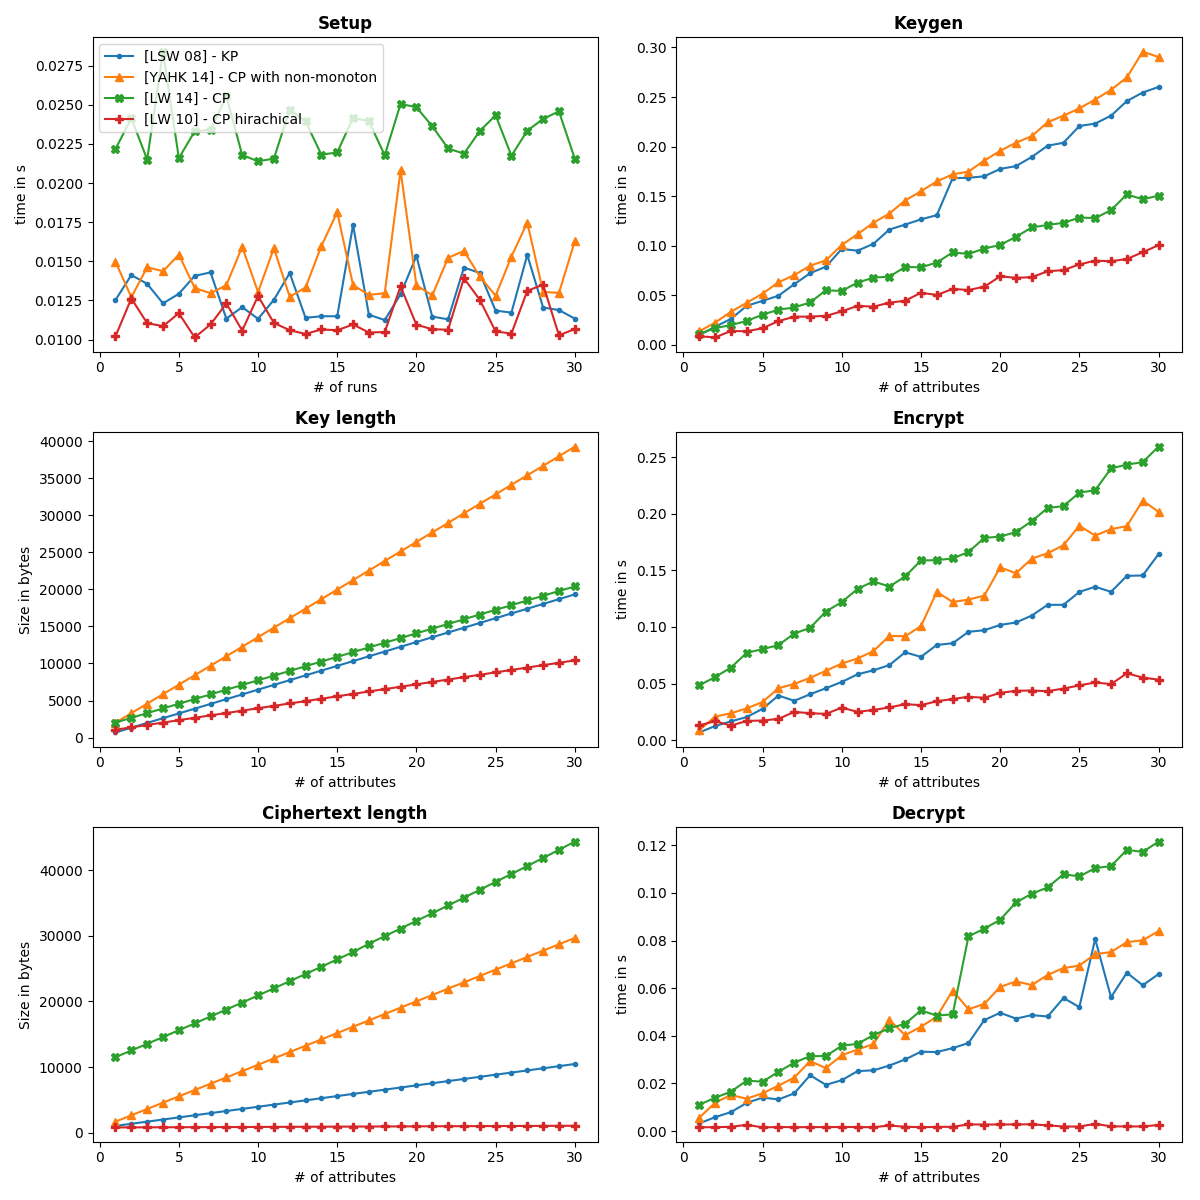
\includegraphics[width=1\linewidth]{img/basic_abe_comparisons.png}
    \caption{Performance and scalability comparison between the chosen schemes with increasing number of attributes. The policy for each new attribute $a_k$ with $a_k \in A$ was defined as $\bigwedge\limits_{a \in A}^a a$. Key generation relates to the creation of users key pairs given an access policy or attribute set.}
    \label{fig:basic_abe_comparison}
\end{figure*}

The  benchmark show in figure \ref{fig:basic_abe_comparison} is executed with a constant size message $m \in G_T$ on a Intel(R) Core(TM) i7-6500U CPU @ 2.50GHz with 16 GB RAM. For the setup was executed 30 times. Here we can see how long the time varies to find suitable curve parameter to initialize the pairing. The other runs are executed with increasing number of attributes. The policy that is used to create the ciphertexts and the user keys in the case of KP-ABE is defined as $\bigwedge\limits_{a \in A}^a a$ where $A$ defines the set of attributes. 

Notable about the comparison in figure \ref{fig:basic_abe_comparison} is that while \ac{KP-ABE} (LSW08) was expected to have the biggest overhead in key generation compared to the \ac{CP-ABE} schemes. This turned out to be not true. It seems more like the time complexity and runtime of the different algorithms surly depends on the design of the scheme. Here we can say that each of the schemes have a linear overhead in runtime. While a constant runtime is only achievable by the HABE scheme the other schemes show a linear time complexity. The HABE scheme in general shows the best overall performance. 
% But it must also be noticed that we specifically excluded attribute authority key generation. 

Due the great performance and the coverage of the most of the requirements of the hierarchical attribute based encryption technique, the field of multi-authority attribute-based encryption will be evaluated in more depth. Regardless of the great scalability of the \ac{HABE} it comes with a non negotiable disadvantage. The root master and the top level domain master have both global decryption power. For each user regardless of the company affiliation the administrator of the system will always be able to decipher ciphertexts of each users. This would break end-to-end encryption. So clearly we would favor solutions that support different attribute authorities so that each company can administer their own domain separately from each other, but it is also desireable that the root, while being able to bootstrap new attribute authorities, is not able to decipher any ciphertext. 

% \ac{MA-ABE}
\subsection{Multi-authority attribute based encryption}
In this section the field of Multi-authority attribute-based encryption (\ac{MA-ABE}) will be evaluated more deeply with respect to all requirements of section \ref{sec:requierements}. 

Another notable technique recently used by \cite{yang2013dac}, \cite{wu2017security}, \cite{li2017two} and \cite{wang2011hierarchical} is \textit{proxy de-/reencryption}. It is motivated by the fact that mobile devices often don't have much computing resources so that the server may help the clients for decryption. The main idea is that the server does the preprocessing of the encrypted text given paramteres by the user. In the end the preprocessed encrypted content will be easily computable by the edge device. The cural fact is that the server will have no knowledge about the plaintext but rather helps the user on decryption or reencryption. 

In the following the different sub topics of \ac{MA-ABE} will be described, analyzed given the requirement set and finally evaluated based on their perforamnce and scalability. 

\subsubsection{Introduction into Multi-Authority Attribute-based Encryption}
Chase 2007 \cite{chase2007multi} was the frist known to introduce the first \ac{MA-ABE} schemes. In her paper she describes the process on how to derrive a multi-authority attribute-based encryption scheme vom the single authrotity schemes. 

The collussion resistance criteria in \ac{ABE} implies that any data owner needs to encrypt under attributes in such kind that the ciphertext is independent of any users specific identifiers. Any user could in theory decrypter the ciphertext if he holds the fullfilling attribute set. While chase's scheme also used bilinear maps it main security was based on interpolation and the fact that no underdefined linaer equation system could definitly be solved\footnote{For \ac{LSSS} matrix are based on the same assumption.}.  

Colluding users can not decrypter any cipher text and the plain text is encrypted using a blinded master secret. The blinding factor is then implemented in the policy so that any user satisfying this policy can restore the blinding factor and so revocer the plaintext. 

In the next step each user is given blinded attribute private keys so that when used on decryption the plaintext is still blinded with the user specific identifier. Using pairings this identifier can be substituted and the plaintext gets revealed. 

Two cural disadventages where not respected by chase in her initial scheme. First the \ac{CA} had global decryption power. It needed to issue each \ac{AA} a specific seed so that on using this seed in a pheudo random generator the \ac{CA} knew what random value would be calculated. This was importent since the \ac{CA} need to isse the user his private key which combined with the private attribute keys from the \ac{AA} would reveal on decryption the unblinded plaintext. 

Chase improved her scheme 2009 in \cite{chase2009improving}. Now all \ac{AA}s will do a n-party key exchange to distribute the secret seeds with each other. Agreeing on a well known value the \ac{CA} was no longer needed and as long $N-2$ \ac{AA}s are not colluding with each other the secret remained secure. 

The other disadventage, that was will present in the updated scheme, was that no new \ac{AA} could be added after system inizialisation since it would trigger a new system inizialisation and distribution of the master secret. 

The lack of addition new attribute authorities and the missing revocation scheme made chases scheme impractical for further evaluations but give a good introduction the fitfalls of \ac{MA-ABE} schemes.

\subsubsection{Hirachical \ac{ABE}}
\label{sec:HABE}

\begin{figure*}[!ht]
\centering
    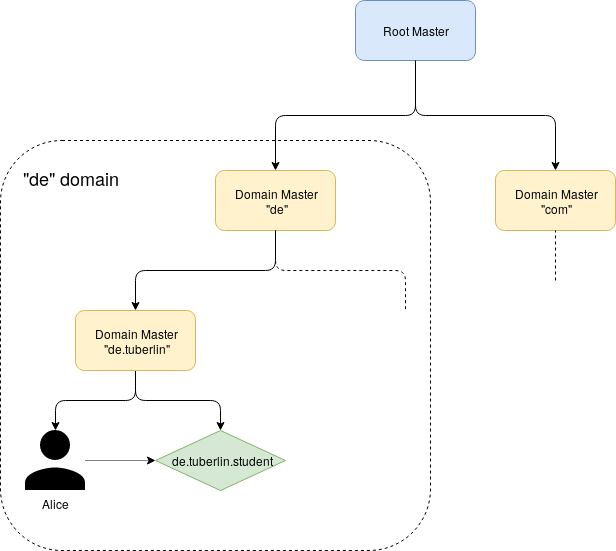
\includegraphics[width=0.5\linewidth]{img/HABE.png}
    \caption{Structe of hirachical attribute-based encryption systems}
    \label{fig:habe}
\end{figure*}

Hirachical Attribute-Based encryption (\ac{HABE}) takes the key delegation one step further. It is sourly designed arround the idea that if a private key exist that have a certain access power, it is possible for the key holder to deletate a subset of his access power to a new instance. By nature follows a hirachical structure where each user could administrate an own subdomain. Here many use cases for cloud computing as well as cloud storage system emerged. \cite{Wang:2010:HAE:1866307.1866414}. While some works also take revocation into design a cural requirement is still missing.

As displayed in figure \ref{fig:habe}, which is based on the approach in \cite{wang2011hierarchical}, the root master summarized the global decryption power of the system and can set up new domain masters (attribute authorities). They on the other hand can delegate a subset of decryption power to a sub domain master. Each domain master can administer users and attributes.

Hirachical \ac{ABE} is the predecessor of Multi-Authority Attribute based encryption. The differences can be summarized by the following points: In \ac{MA-ABE} each user is assigned to a specific attribute authority. This must not be the case in \ac{HABE}. \ac{HABE} is tree-like orientated. Starting from the root node each following authority will have a subset of decryption power as its respectiv parent. 

\cite{Wang:2010:HAE:1866307.1866414} formalized this approach using \ac{CP-ABE}, which was later extended in \cite{wang2011hierarchical}. While implementing a revocation scheme, they depend on an access policy present in \ac{DNF}, which might not always be possible without using negation. 

A hirachical strcture and a delegation of decryption power would, as already mentioned, imply that the root master has global decryption power which is not desired \req{C4}. We want to design a system in which each domain is seperated is term of key generation from each other. That means that there is no top level domain which has global decryption power, rather we want to have a system where each subdomain creates its down keys and administrataes thier own attributes but that is still a part of a bigger system so able to interact with other domains.  
\todo{Reformulate}

\subsubsection{Decentralized attribute-based encryption}
\label{sec:DABE}
Both issues where addressed with the sub topic of \textit{decentralized attribute based encryption} (\ac{DABE}). As the name indicates \ac{DABE} does not need a \ac{CA} managing the setup of additional \ac{AA}s. This ecosystem is self sustaining in the form that each entity can become an \ac{AA} if needed and start issuing new attributes to users. 

Some form of centralization must be still preserved. The global paramter for example needs to be known to each new entity and each user usally need to get a unique global identifier to be identified among the set of users. Also attributes need to be somehow syncronized since the set of attriubte identifier usally need to be non intersecting across different domains. All this information could be published by a public bullitin board and was first proposed by \cite{lewko2011decentralizing}. 

Revocation in such system remains an open issue. Since no central authority manages all users, no authority can be in charge of revocing them. An authroity could revoce its issued attributes but only in an indirct fassion since decentralzied systems are build around the idea that nodes can go offline at any time. If an authority would go offline as soon at it received the revocation request the revocation procedure would never trigger. 

Cui and Deng showed in \cite{cui2016revocable} that such a system could exist. Each key and ciphertext got a liveness assigned that is active for a certain time periode. After the time periode expired all keys need to be reissed by each \ac{AA}. Indirect revocation happens by simply not reissuing a user certain attribute keys. This sytem is implemented in the comparison in \ref{sec:ma-comparison}.

The question remains if such a system would be practically applicable since each cipher text needs to be reuploaded in each time periode. Revocation in decentralized attribute based encryption remains an open issue.

\subsubsection{Efficient Data Access Control for Multi-Authority Cloud Storage}
The most explored field in \ac{MA-ABE} is the Efficient Data Access Control for Multi-Authrotity Cloud Stroage (\ac{DAC-MACS}) family \cite{yang2013dac}). First instroducted by Yang \textit{et. al.} 2013 it desribes an efficient, revocable \ac{MA-ABE} scheme based on \ac{CP-ABE} and using proxy encryption on decryption and reencryption. Furhter this scheme features a large attribute universe, adding \ac{AA}s on the running system and serves with a \ac{CA} that has no global decryption power. In sort \ac{DAC-MACS} satisfy all the non-optional requirements.

\ac{DAC-MACS} elliminates the need for the global decryption power of the \ac{CA} by issuing $k$ ciphertexts: One per \ac{AA}. \footnote{If the ciphertext does not require any attributes of an specific authority it does not have to create a ciphertext for this domain.} It does not require any coordination between authorities which enables to add new \ac{AA}s at runtime without recreating the user keys. This scheme also includes features for efficient revocation while it claims to maintain forward and backward secrecy.

\ac{DAC-MACS} is not collusion resistance on attribute revocation under the active attack model. The scheme \ac{NEDAC-MACS} (New Extended \ac{DAC-MACS}) shows and solves this vulnerability \cite{wu2017security}. Recent studies introduce a more efficient, scalable and secure approaches such as \ac{MAACS} \cite{li2016secure} and \ac{TF-DAC-MACS} (Two-Factor \ac{DAC-MACS})\cite{li2017two}. 

All the \ac{DAC-MACS} schemes are structed in roughly the same way. They usally describe six different entities:

\begin{enumerate}
	\item \textbf{Certificate/Central Authority (\ac{CA})} The purpose of the \ac{CA} is to issue user their global identifier (\ac{GID}). Furhter they bootstrap the different \ac{AA}s. The \ac{CA} remains trusted but do not have any decryption power in the system. 
	\item \textbf{Attribute Authority (\ac{AA})} A attribute authority administers their domain. Issues attributes and their respective privat key to the user. They only accept a user if his \ac{GID} is signed by the \ac{CA}. 
	On revocation they will need to update the users secret keys as well as the ciphertext encrypted with the revoked attribute key. \ac{AA}s are assumed to be trusted but can be compromised by an adversary.
	\item \textbf{Server} The purpose of the server is to help the user with proxy re- and decryption. If an \ac{AA} broadcast a revocation of an attribute, the server may download all related ciphertexts from the \ac{CSP} to update them with the new attribute. 
	Further, the user may give the server his attribute privat keys so that the server can pre compute the ciphertext. Usally the thread model for the server is honest-but-curious. Please note, that the \ac{CA} and the server are two seperated entities that do not cooperate.
	\item \textbf{Data owner} The data owner are usally users who want to encrypt content with under a specific access policy. To do so they use the publically available public keys pinned on the public bullition board of the respective \ac{AA}. Data owner do not have any knowledge about \ac{GID} or user groups in the system. After encryption they update the encrypted content to the \ac{CSP}.
	\item \textbf{Cloud storage provider (\ac{CSP})} The cloud storage provider are assumed to be untrusted while they still follow the protocol. That why they only receive encrypted data. They only purpose is to store the ciphertext and make them puplically available. No authentication checks are needed.
	\item \textbf{Users} Users exist in two groups: Revoked and non-revoked. Revoked user try to collude with each other to get a higher level of decryption power. They download the files of the \ac{CSP} and try to decrypter them. Only if they attribute set matches the policy of the ciphertext they will be able to decrypt the file. 
	Revoked user on the other hand try to still decipher ciphertext. In some cases they try to collude with non-revoked user to intercept the key update key to restore their decryption rights. 
	User are in general untrusted.
\end{enumerate} 

\ac{TF-DAC-MACS} counts as the most advanced \ac{DAC-MACS} scheme providing non global decryption power, secure revocation channels and both backward and forward secrecy. In addition \ac{TF-DAC-MACS} introducted the two factor authentication where data owner can issue and revoce \textit{authentication keys} to and from users. This adds an additional layer of security. In total \ac{TF-DAC-MACS} archives still better performance then the other \ac{DAC-MACS} schemes probiding constant decryption and encryption overhead. 

We will compare the basic proposal of \ac{DAC-MACS} with \ac{TF-DAC-MACS} in the comparison. 

\subsubsection{Comparison}
\label{sec:ma-comparison}
\begin{table*}[!ht]
\centering
\begin{tabular}{l 					| l 									| l 									| l 					| l}
									& \thead{LTXWC 16\\(TF-DAC-MACS)\cite{li2017two}} & \thead{YJ 14\\(DAC-MACS)\cite{yang2013dac}} & \thead{LW 14\\ (HABE)\cite{wang2011hierarchical}}	& \thead{CD 16\\(DABE)}\cite{cui2016revocable} \\
\hline
\thead{Scheme}						& \makecell{CP (DAC-MACS \\ without proxy \\ 
									  decryption, 
									  with \\ two-factor \\ authentication)} & \makecell{CP (DAC-MACS \\ 
									  										  with proxy \\ decryption)} 			& CP (Hirachical) 		& CP (Dezentralized)		\\ 
\hline
\thead{Revocation}					& Direct 								& Direct 								& Direct 				& Indirect					\\
\hline
\thead{Security scheme}				& Biliniear maps 						& Binilnear maps 						& Biliniear maps 		& Biliniear maps 			\\
\hline
\thead{Expression of \\ access policy} & n-of-n threshhold					& LSSS		 							& DNF 					& LSSS matrix 				\\ 
\end{tabular}
\caption{Scheme description. }
\label{tab:comparison_ma_abe_overview}
\end{table*}
\begin{table*}[!ht]
\centering
\begin{tabular}{l 	| l										| l 									| l 					| l}
					& \thead{LTXWC 16\\(TF-DAC-MACS)\cite{li2017two}} & \thead{YJ 14\\(DAC-MACS)\cite{yang2013dac}} & \thead{LW 14\\ (HABE)\cite{wang2011hierarchical}}	& \thead{CD 16\\(DABE)}\cite{cui2016revocable} \\
\req{C1}			& Yes									& No 									& Yes 					& Yes 						\\
\req{C2}			& Yes									& Yes 									& Yes 					& Yes 						\\ 
\req{C3}			& Yes									& Yes 									& No 					& Yes 						\\ 
\req{C4}			& Yes									& Yes 									& No 					& Yes 						\\ 
\req{C5}			& Yes									& Yes 									& Yes 					& Yes 						\\ 
\req{C6}			& Yes 									& Yes 									& Yes					& Yes						\\
\req{C7}			& Yes									& Yes 									& No 					& Yes 						\\
\req{C8}			& Yes									& Yes									& Yes					& Yes-						\\
\req{O1}			& No 									& No 									& No 					& No 						\\
\req{O2}			& No 									& Yes									& Yes					& Yes						\\
\end{tabular}
\caption{Requirements comparison of the implemented schemes}
\label{tab:ma_abe_comparisons}
\end{table*}


\begin{figure*}[!ht]
\centering
    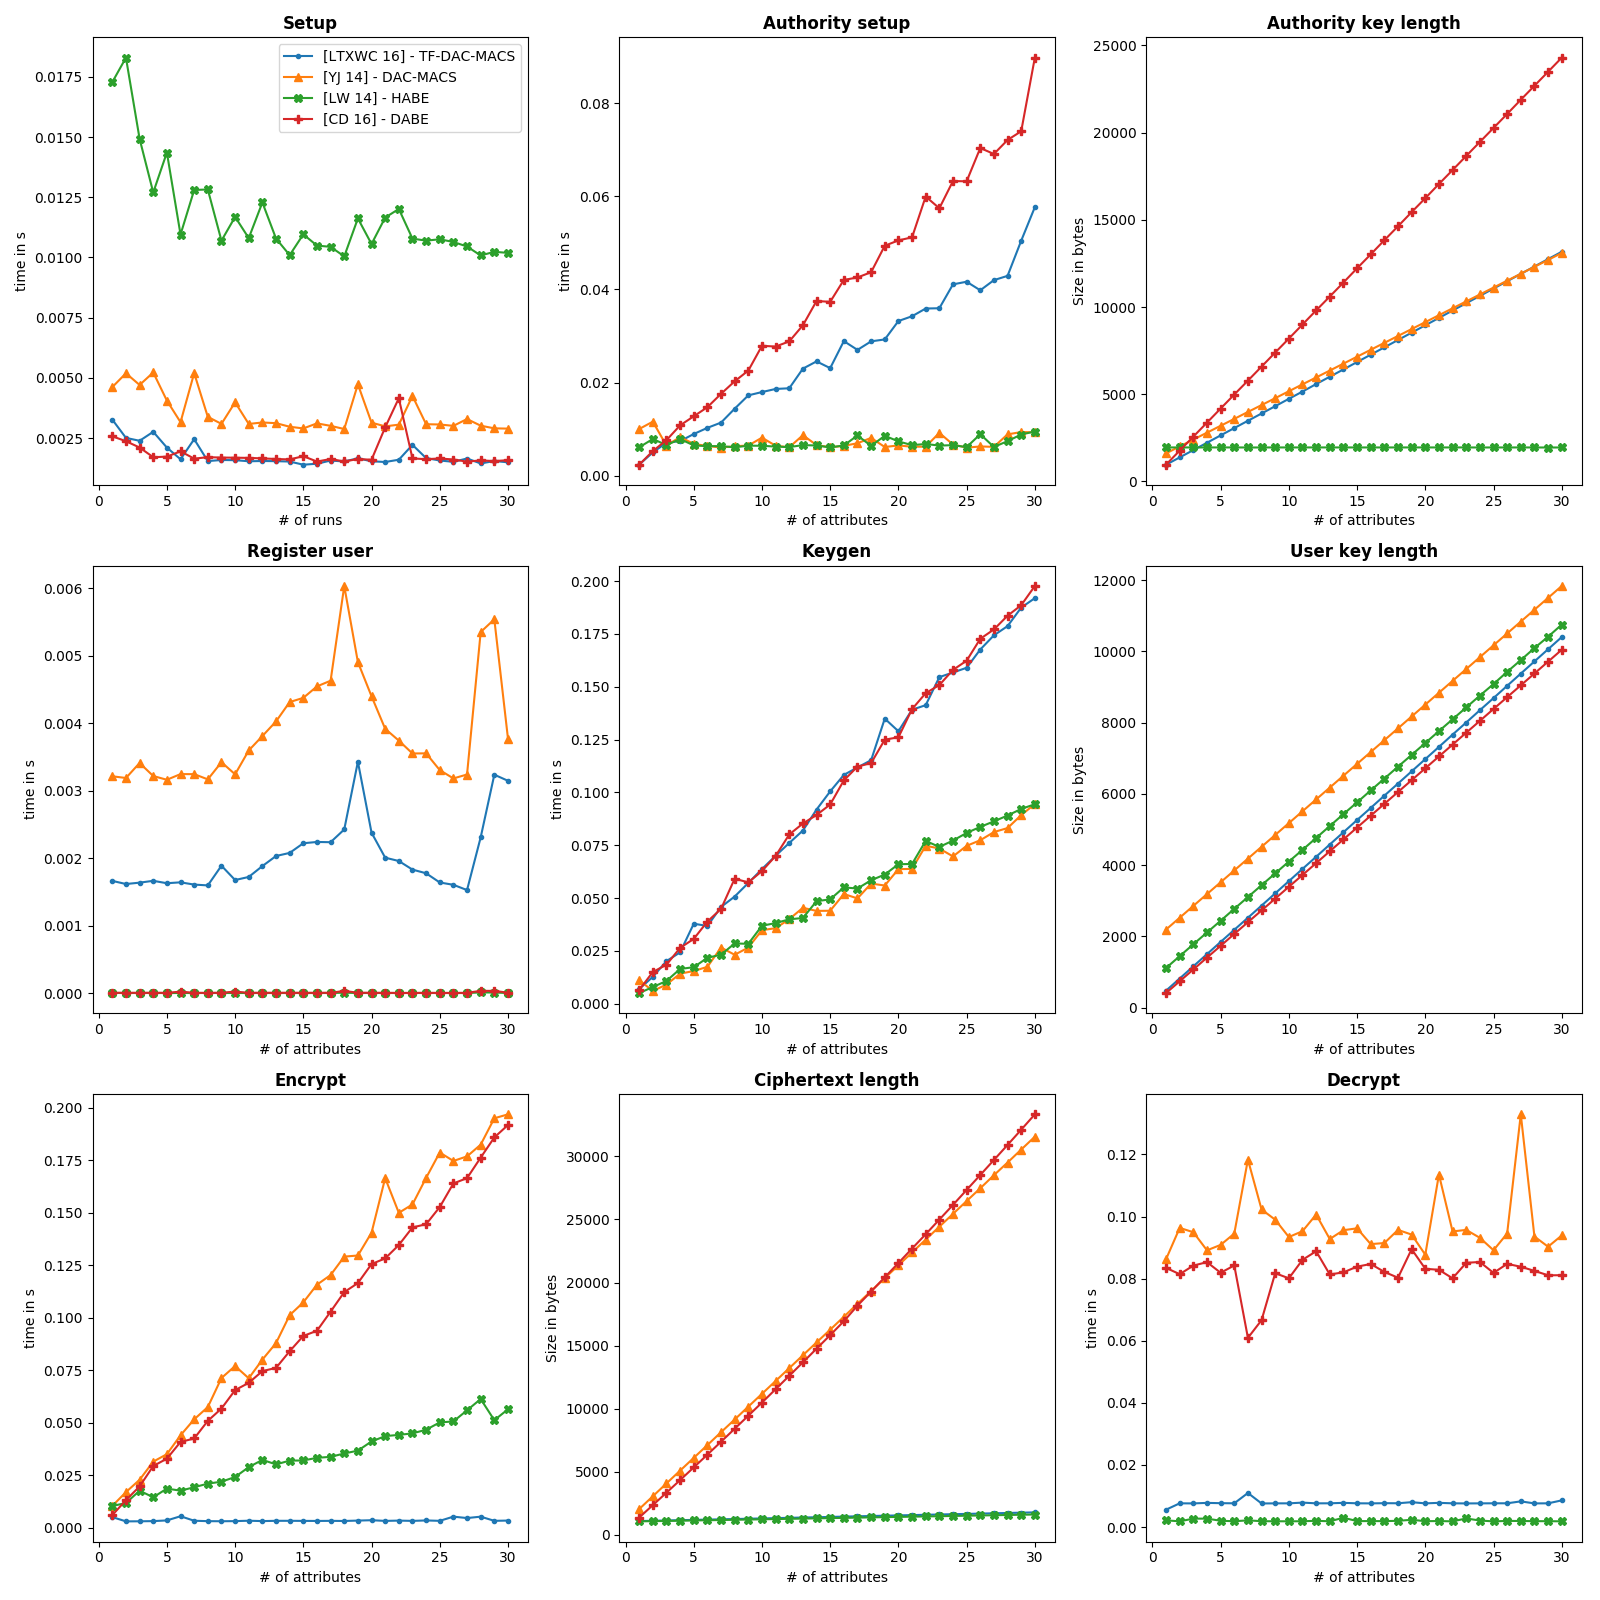
\includegraphics[width=1\linewidth]{img/maabe_comparisons.png}
    \caption{Performance and scalability comparison}
    \label{fig:maabe_comparison}
\end{figure*}

To compare the sub topics of \ac{MA-ABE} we need to extend the charm framework with an implementation of \ac{DABE}, \ac{HABE} and \ac{TF-DAC-MACS}. \ac{DAC-MACS} on the other hand exisited in the farmework already. 

In general we extracted five steps that each \ac{MA-ABE} scheme need to provide in some form. 
\begin{enumerate}
	\item \textbf{Setup:} The global setup phase where public paramter are settled.
	\item \textbf{Authority Setup:} \ac{AA}s can register themself to the central authority (if any) and compute their secret keys. Usally, the attribute secret keys are generated as well. 
	\item \textbf{Register User:} In the \ac{DAC-MACS} schemes user receive public and private key components. They are used for proxy decryption so that the server can help the user on decryption without revealing the plaintext. To do so the server generates a \textit{decryption token} which is encrypted with the users public key. Other schemes just assign the user a \ac{GID}. 
	\item \textbf{Kegen:} Attributes are assigned to user and the respective secret keys are generated.
	\item \textbf{Encrypt:} The cipher text is encrypted by the data owner under an access policy.
	\item \textbf{Decrypt:} The user (with the help of the server) decrypts the cipher text and revocers the secret message m. 
\end{enumerate}

This steps are shown and compared in \ref{fig:maabe_comparison}. As it turns out no scheme can be defined as the most performant or most scalabe one. All schemes performace roughly equally good. Some could argue that \ac{DAC-MACS} performed the worst, then \ac{DABE}, then \ac{TF-DAC-MACS} and the best performance has \ac{HABE}. 

However, for pratical usage especially the encryption and decryption performance is cural. There only \ac{TF-DAC-MACS} has an constant overhead while all other schemes are linear. If we further have a look at the table of requirements \ref{tab:ma_abe_comparisons}, we see that only two schemes satisfy all of the requirements: \ac{TF-DAC-MACS} and \ac{DABE}. \ac{DABE} profits also from the fact that it has a more fine grant access control then \ac{TF-DAC-MACS}. However, its revocation scheme is the disadventage that leave us with \ac{TF-DAC-MACS} as our final candidate. As mentioned in section \ref{sec:DABE} the implemented scheme uses indirct time-based revocation, which forces data owner to periodically reencrypt and reupload thier content. This is in a cloud storage system not really applicable. 

The comparison of \ac{TF-DAC-MACS} with other schemes of the \ac{DAC-MACS} family was left out in this work, since it was already done in the \ac{TF-DAC-MACS} paper \cite{li2017two}. Here some could easly see that \ac{TF-DAC-MACS} is currently the most performant scheme in the \ac{DAC-MACS} family.  

\section{Thread Model}

TF-DAC-MACS describes six entities which will have different trust levels in our design. In the following the certificate authority and central server are merged, as well as the user and data owners are merged. 
\begin{itemize}
	\item The \textbf{Central Server} is assumed to try to break into the client communication. It might provide false information or wrong states to trick any identity to provide sensitive content. However, the central server will cooperate and will only deviate from the protocol if some advantage could be gained. Simply denying the cooperation – and so disrupting the service - does not belong to the goals of the central service. The central service does not cooperate with other malicious entities. 
	\item Each \textbf{Attribute Authority}’s goal is to access and eve drop content that is encrypted with attributes outside if its domain.  This distrust can be leveraged by a trust relation ship, where two attribute authorities can explicitly agree to trust each other. This mutual trust relation indicates that an trusted attribute authority is assumed to provide only truthfully information to the other trusted authority. Again it is assumed that an attribute authority does not cooperate with other malicious entities and that it will follow the protocol.
	\item \textbf{Cloud Storage Provider} are simply assumed to be honest-but-curious. They follow the protocol by try to decrypt content if possible. A cloud storage provider is separated from the other system and does not cooperate with any other malicious entity.  
	\item \textbf{Users} are untrusted. They try to collude with each other to achieve a higher level of decryption power. That means that they will exchange private attribute and two factor keys. However, it is assumed that they will not sell a decryption black box so that other external, unauthorized or revoked users use the black box to access sensitive content. 
\end{itemize}

This thread model is different from that proposed in TF-DAC-MACS. Here the central server and certificate authority are also semi-trusted. This is compensated by leveraging the trust level of the attribute authorities by introducing the trust-relationship. In TF-DAC-MACS a lot of trust is rooted in the certificate which was issued by the trusted certificate authority. In a real life system the trust of the certificate authority needs to be deescalated, since it is usually controlled by the same entity as the central server. To do so, for each certificate validation a second channel needs to be established: One to the issuer and one to the subject of the certificate, asking both for the validity of the certificate. 

% summary
\section{Summary}
In the past sections we evaluated the path from the classical rekeying scheme to multi-authority attribute based encryption. We reviewed different more topics in secure group communication and motivated the direction of why attribute based encryption might be a more suitable scheme. Finally, we showed that multi-authority attribute based encryption is more appropriate for the secure cloud storage systems domain. In that research area we found TF-DAC-MACS which finally satisfies all the requirements and provides acceptable scalability. 

In comparison to the classical rekeying scheme we expect better performance on en- and decryption when scaling up the number of clients. It further have to be noticed that the performance improvements of ABE in comparison to RSA depend surely on the selected use case. If group will be formed that can be described completely by a low number of attributes ABE will be more efficient. However, if groups are created that can not easily be described by a low number of attributes, ABE will perform with the same overhead as the current scheme. 

Whether this assumption holds true in practice and if the day-to-day use cases of the user are sufficient to provide the promised performance boost will be evaluated in the following sections.

% Implementation
\chapter{Implementation}
As evaluated in the last sections we will proceed to implement TF-DAC-MACS with small adaptions for a practical secure cloud storage system. To do so five entities need to implemented into our distributed system:  

\begin{itemize}
  \item \textbf{Central Server} does the initial setup of the global public parameter used in the later process. It publishes this information on a public bulletin board. Further, the CA is the central entry point to trigger and permit AA creations. It audits the \textit{Authority Identifier} (\ac{AID}) provided by the AA and which should be unique in this system. 

Further, the CA functions as a \textit{Certificate Authority}. It issues a certificate for the GID and RSA public keys of the user. This certificate can be revoked so that the user is not able to obtain new secret keys from the AA or other data owners.
The CA is also the central service that provides all necessary information to the client. Such as public attribute keys, encrypted user private attribute keys and certificates.
 The Central Server is honest-but-curious.
  \item \textbf{Attribute Authority (\ac{AA})} creates the secret keys for its attributes. Attributes are prefixed with the \ac{AID} to ensure uniqueness among the attribute universe. AAs are also untrusted but never collude with users. They have decryption power in their domain. 
  \item \textbf{Cloud Storage Provider (\ac{CSP})} The cloud storage provider provides storage to save the encrypted files. If an cipher text update is needed the CSP updates the cipher text accordingly. 
  \item \textbf{Users} download and decipher ciphertext. They receive attribute secret keys from the AA, GID and certificates from the server and two factor keys from the data owners. The CSP is honest-but-curious as well.
  \item \textbf{Data owner} are specifications of users who can issue two-factor keys to other users. The so called \textit{Two-Factor Key} (\ac{2FA}-Key), adds an additional security layer to the cipher text. It restricts the access to the encrypted plain text to a even smaller select user group.  
\end{itemize}

In the following sections, the different phases setup, encrypt, decrypt, attribute revocation and authentication key revocation are shortly explained. Please note that for any scheme details we referrer to the TF-DAC-MACS \cite{li2017two} paper .

\section{Setup}
\begin{figure}[!ht]
\centering
    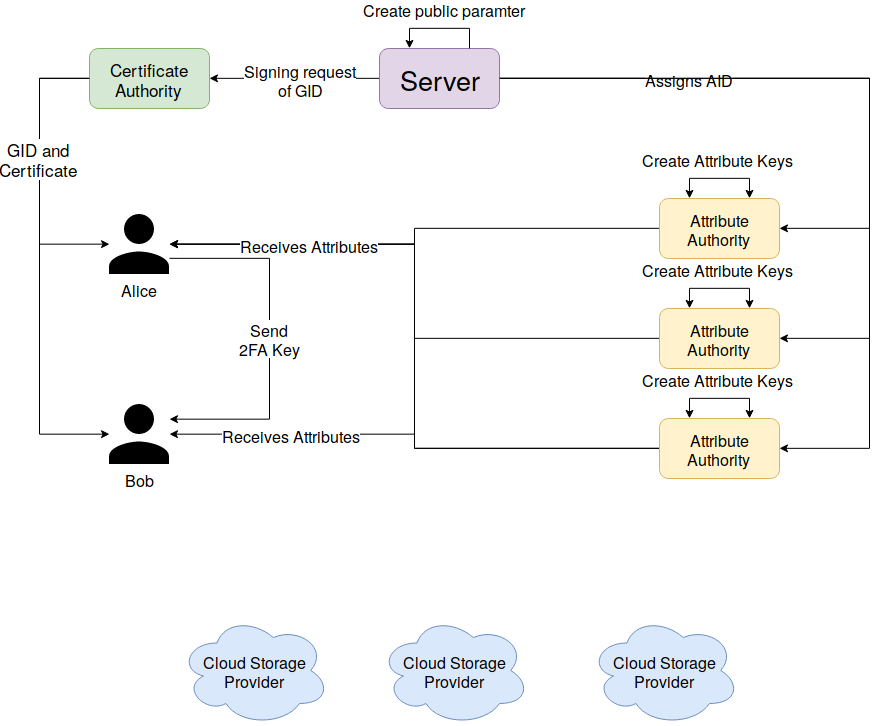
\includegraphics[width=\linewidth]{img/TF-DAC-MACS-overview-setup.png}
    \caption{Setup phase}
    \label{fig:tfdacmacs-setup}
\end{figure}

The setup summarizes the steps described in \cite{li2017two} such as: Setup, user registration, data owner registration, authority setup, key generation and authentication requests. 

The first step is to create the global public parameters on the server. Thous parameter are exposed on a public bulletin board and available for each entity in the system. Since they are required in every step it is assumed that the entity downloaded this information in advance. 

On AA setup the server first generates a new AID. This AID will be mapped to the domain name of this entity. So for example the TU-Berlin will have as its ID: "aa.tu-berlin.de". In this way it is ensured that no AID can double. Further, it would be verifiable via the certificate chain of TLS/SSL that this AID indeed belongs to the TU-Berlin. To do so the certificate coupled with this domain can be verified and then a query to "aa.tu-berlin.de" would lead to the corresponding AA of the TU-Berlin.

The AA is free to generate attribute keys. Attributes also have identifier and values assigned to them. Values and attribute identifier can be any valid string as long as it does not contain any special characters such as ":" or ".". The attribute will have the form of "<AID>.attr.<Attribute\_name>:<Attribute\_value>". For example the major computer science would be displayed as "aa.tu-berlin.de.attr.major:computer\_sience". Each attribute-value pair gets a secret key assigned. The public component for this attribute will be saved in the AA and published on the public bulletin board of the Central Server. 

In the next step, users are registered to the server. They receive the GID and a certificate for this GID. They can use the certificate later on to register to the AA or to authenticate them self to other users. The GID will be the email of the user. After the certificate is approved by the AA, it encrypts the user specific attribute value keys with the public key embedded in the presented certificate and pushes the encrypted attribute value keys to the central server. The user downloads and decrypts this keys. \todo{include registration flow graphic and describe this flow more deeply}

In the final setup, users can issue each other two factor keys so called \textit{authentication keys}. This authentication keys introduce a new layer of security where users can decide who exactly can decipher their plain text. In some cases this may be needed since access policies in ABE describe always a group of user and the exact members of this group remains hidden from the data owner.
 
An example flow to receive the 2FA-Key would look like this: If Bob wants to get an authentication key from Alice he sends an authentication request to the CA addressing Alice and containing his certificate. Alice gets notified about the request, checks the validity of the certificate and creates the authentication key for Bob. She  uses the public key embedded in Bobs certificate to encrypt the private authentication key and uploads it to the CA. Bob downloads the encrypted key and decrypts it. In the later manner, Bob can use this authentication key to authenticate against the cipher text created by Alice. 

The previous steps are summarized in the figure \ref{fig:tfdacmacs-setup}.

\section{Encryption}
\begin{figure}[!t]
\centering
    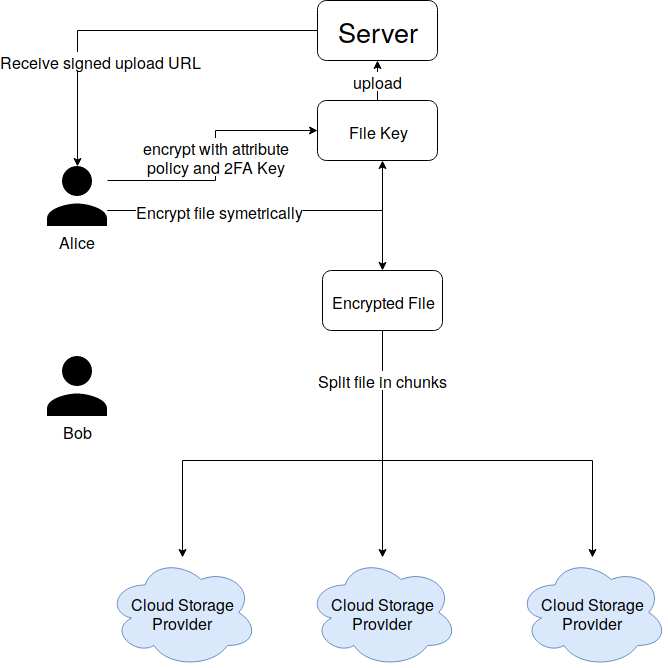
\includegraphics[width=0.7\linewidth]{img/TF-DAC-MACS-overview-encrypt.png}
    \caption{Encryption phase}
    \label{fig:tfdacmacs-encrypt}
\end{figure}

For en- and decryption we will still use the process of encrypting the file symmetrically to create a file key which will then encrypted under the attribute policy. This reduces the size of the content that will be encrypted with ABE to a minimum. Moreover, we can still benefit from the great performance of \ac{AES}. 

To upload a file encrypted under an access policy, Alice first creates the access policy (figure \ref{fig:tfdacmacs-encrypt}). In addition she is also able to encrypt the ciphertext with the authentication key she issued to Bob. \todo{Overwork graphic, might not match}. This results in a random secret $M \in G_T$. She transforms $M$ to a bit-stream and uses this as the key to encrypt the file content symmetrically. Alice uploads the ciphertext and the encrypted content to the CSP. 

\section{Decryption}
\begin{figure}[!t]
\centering
    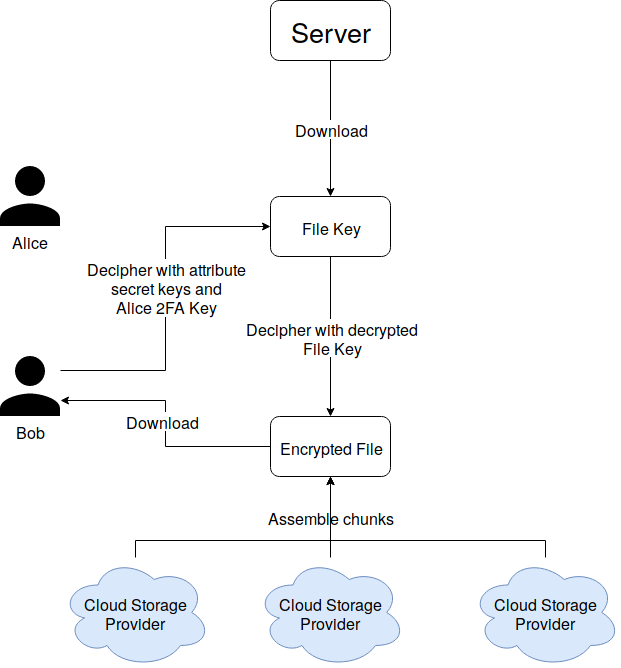
\includegraphics[width=0.7\linewidth]{img/TF-DAC-MACS-overview-decrypt.png}
    \caption{Decryption phase}
    \label{fig:tfdacmacs-decryption}
\end{figure}

On decryption first the ciphertext will be downloaded from the server. If Bob has a matching super set of attributes and the needed 2FA-Key he can recover the file key $m$ and transform it again to a bit-stream (figure \ref{fig:tfdacmacs-decryption})

Next, he downloads the encrypted file from the CSP and decrypts it with the recovered file key.

\section{Revoke attribute}
\begin{figure}[!t]
\centering
    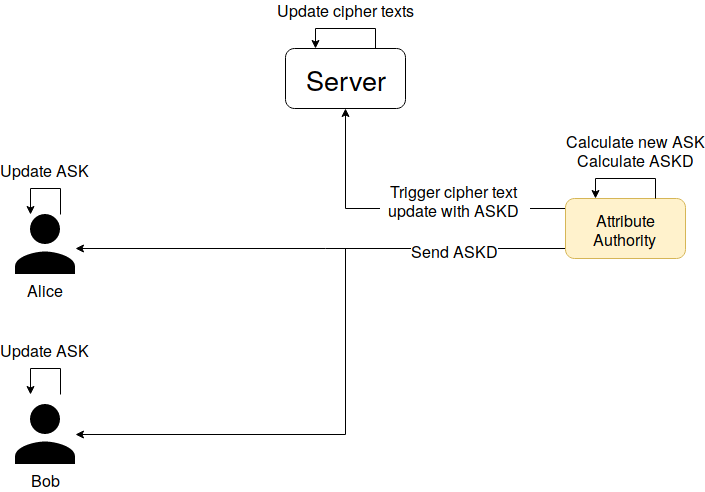
\includegraphics[width=0.7\linewidth]{img/TF-DAC-MACS-overview-revoce-attr.png}
    \caption{Attribute revocation}
    \label{fig:tfdacmacs-attr-revocation}
\end{figure}

As displayed in figure \ref{fig:tfdacmacs-attr-revocation}, a revocation of an attribute key is always triggered by the AA that administers this attribute. It first creates a new secret key for the revoked attribute and calculates for each user owning the old attribute a user-specific delta. This delta is send to each non-revoked user respectively. In addition, the AA calculates a cipher text update key. This is send to the CSP which then in turn starts updating all the cipher text for the new attribute secret key. This operation will not affect the plain text message in any kind. 

\section{Revoke two-factor key}
\begin{figure}[!t]
\centering
    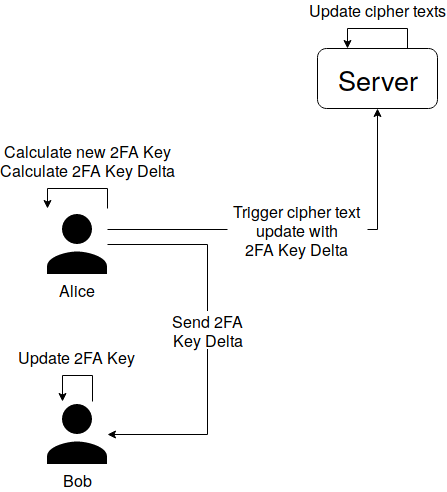
\includegraphics[width=0.6\linewidth]{img/TF-DAC-MACS-overview-revoce-user-key.png}
    \caption{Two-factor key revocation}
    \label{fig:tfdacmacs-user-auth-key-revocation}
\end{figure}

In a similar way as attributes are revoked, 2FA-Keys can be revoked. Alice, as the data owner, starts  by calculating a new two-factor key. She computes the delta to all old two-factor keys she issued and distributes them to all non-revoked users. Finally, she calculates the ciphertext update key and sends it to the CSP. The CSP updates all relevant cipher texts.

\section{Adaptions and Improvements}
While TF-DAC-MACS satisfy all the requirements it fits not perfectly. To make the scheme more usable, the fix contain that each cipher text need to be secured by a two-factor authentication was removed. In addition, the key generation of the attribute is made more dynamic. Now the attributes do not need to be known in the setup phase but can be created dynamically when an AA admin registers a user. Further, we propose a simple technique to break up TF-DAC-MACS n-of-n threshold policy in trade-off for performance. And finally we apply a technique proposed in \cite{bethencourt2007ciphertext} to implement numerical values and comparisons in boolean access formula. 

\subsection{Removing the fix two-factor contain}
To make \ac{TF-DAC-MACS} more practically applicable we removed the fixed two-factor constrain from the encryption, decryption, and cipher update phase. The two factor identifier $\alpha$ is used by the data owner to restrict the access to the content for certain users. 

This leads to the fact that the underlying \ac{ABE} schemes looses some of it expressiveness. The zero knowledge of the data owner on which individual is able to decrypt the cipher text is broken with the two factor part. Here each user, who wants to decrypt the encrypted content, needs to make an \textit{authentication request} to the data owner to receive the corresponding decryption key. To restore the possibility to let an unknown user group decrypt the cipher text, we make the two factor part optional. To do so we adapted encryption, decryption and cipher text update. The authentication key update will be ignored since it makes no sense to apply it on a non existing authentication key. 

\begin{itemize}
\item \textbf{Encryption:} 
We only need to update the $C_3$ part of the cipher text since it is the only one containing the two factor component $\alpha$.

The original $C_3$:
$$
C_3 = \Big( \prod_{v_{aid_{i}, j}\in W} g^{y_{aid_{i}, j}} \Big)^{s + \alpha} 
$$
is adapted to:
$$
\widehat{C}_3 = \Big( \prod_{v_{aid_{i}, j}\in W} g^{y_{aid_{i}, j}} \Big)^s
$$ 
In addition we will remove $oid$ from the ciphertext description since it referrers to the data owner ID which is only needed on authentication key update.

\item \textbf{Decryption:}
$SK_W = \prod_{v_{aid_i,j} \in W} SK_{v_{aid_i,j}}$ and $UPK_W = \prod_{v_{aid_i,j} \in W} UPK_{v_{aid_i,j}}$ remain defined in the same was as defined in the paper. 

On decryption the user does not need to generate $UPK_W$ and $SK_{uid, oid}$ anymore. The decryption equation is updated to:

$$
m = \frac{C_1 \cdotp e(H(uid), \widehat{C}_3)}{e(C_2, SK_W)}
$$

Note that the original decryption equation results in the above equation when the two factor part is deducted.

\begin{equation}
\begin{split}
m &= \frac{C_1 \cdotp e(H(uid), C_3)}{e(C_2, SK_W)e(SK_{uid, oid}, UPK_W)} \\
  &= \frac{C_1 \cdotp e\Big(H(uid), \Big( \prod_{v_{aid_{i}, j}\in W} g^{y_{aid_{i}, j}} \Big)^{s + \alpha} \Big)}{e(C_2, SK_W)e(H(uid)^\alpha, \prod_{v_{aid_i,j} \in W} UPK_{v_{aid_i,j}})} \\
  &= \frac{C_1 \cdotp e\Big(H(uid), \Big( \prod_{v_{aid_{i}, j}\in W} g^{y_{aid_{i}, j}} \Big)^{s + \alpha} \Big)}{e(C_2, SK_W)e(H(uid)^\alpha, \prod_{v_{aid_i,j} \in W} g^{y_{aid_i,j}})} \\
  &= \frac{C_1 \cdotp e\Big(H(uid), \Big( \prod_{v_{aid_{i}, j}\in W} g^{y_{aid_{i}, j}} \Big) \Big)^{s + \alpha}}{e(C_2, SK_W)e(H(uid), \prod_{v_{aid_i,j} \in W} g^{y_{aid_i,j}})^\alpha} \\
  &= \frac{C_1 \cdotp e\Big(H(uid), \Big( \prod_{v_{aid_{i}, j}\in W} g^{y_{aid_{i}, j}} \Big) \Big)^{s}}{e(C_2, SK_W)} \\
  &= \frac{C_1 \cdotp e\Big(H(uid), \Big( \prod_{v_{aid_{i}, j}\in W} g^{y_{aid_{i}, j}} \Big)^{s} \Big)}{e(C_2, SK_W)} \\
  &= \frac{C_1 \cdotp e(H(uid), \widehat{C}_3)}{e(C_2, SK_W)}
\end{split}
\label{eq:2faRemoval}
\end{equation}

As shown, no security is threatened since we end up at the same equation as we would if we had the two factor part included. 

\item \textbf{Attribute revocation:}
The cipher text update key is adapted from

$$
CUK^{ID_W}_{v_{aid_i,j}} = (g^s \cdotp g^\alpha)^{y'_{aid_i,j} - y_{aid_i,j}}
$$

to 

$$
\widehat{CUK}^{ID_W}_{v_{aid_i,j}} = (g^s)^{y'_{aid_i,j} - y_{aid_i,j}}
$$

$\widehat{C}'_3$ now computes as 

\begin{equation}
\begin{split}
\widehat{C}'_3 &= \widehat{C}_3 \cdotp \widehat{CUK}^{ID_W}_{v_{aid_i,j}} \\
&\cdotp \Big( \prod_{v_{aid_{t}, j}\in W, v_{aid_t, j} \neq v_{aid_i,j}} g^{y_{aid_{i}, j}} \Big)^{r} \cdotp (g^{y'_{aid_i,j}})^{r} \\
&= \Big( \prod_{v_{aid_{t}, j}\in W, v_{aid_t, j} \neq v_{aid_i,j}} g^{y_{aid_{i}, j}} \Big)^{s + r} \cdotp (g^{y'_{aid_i,j}})^{s + r}
\end{split}
\end{equation}

It can be shown that $C'_3$ computes to the message $m$ in the same way as shown in equation \ref{eq:2faRemoval}.

\item \textbf{Authentication update:}
Nothing need to change since cipher text do not contain authentication components. 
\end{itemize}

\subsection{Dynamic Secret Key Generation}
Another small adaptation in the \ac{TF-DAC-MACS} scheme was that the attributes for each \ac{AA} does not have to be known on AA initialization. They can as well be created on each users key generation. This reduces the universe of possible attribute values to thous who are actually needed.

\section{Extension To DNF-Policy}
One big advantage of TF-DAC-MACS is its constant size cipher text. It archives this by only allowing n-of-n threshold policy. This means that a data owner is only allowed to create \textit{AND} policies to encrypt his content. However, extending this scheme to n-of-m threshold policy is not trivial. To not break any security constrains we decided to just upload multiple versions of the same cipher text encrypted under different policies. Now, an user only needs to decipher one version of the cipher text to recover the encrypted content. 

Using this approach we enable access policies in disjunctive normal form (DNF) for the trade-off of linear cipher text overhead and linear overhead on cipher text updates (both scaling with the number of disjunctions).

\section{Numerical Attributes}
As described in \cite{bethencourt2007ciphertext} we could display numeric values in binary. Each number $x$ is composed of $\lceil log_2(x) \rceil$ attributes. Each of this attributes relate to either a $1$ or $0$ in one position in the binary number representation of $x$. So for example the number $5$ in binary would be displayed as $0101$ and its attribute would be: $x:0***$, $x:*1**$, $x:**0*$ and $x:***1$. 

If a user now wants to create a policy where he challenges a number $x$ to be greater or equal to $3$ he creates a policy: "$(x:1*** or (x:*1** or (x:**1* and x:***1))$". Analogous the policy for $x$ smaller than $4$: "$(x:0*** and (x:*0** or (x:*1** and x:**0* and x:***0))$".

Disadvantage of this representation is that it is limited in space. To display a 32-bit number we must issue 64 attribute values and maintain 64 attribute value keys. 


\section{Technologies}
To develop the first prototype of the system defined previously we will use the following technology stack:

\begin{itemize}
  \item \textbf{Spring boot}
  \item \textbf{Docker}
  \item \textbf{jPBC} \cite{ISCC:DecIov11}
  \item \textbf{...}
\end{itemize}
\todo{write me}

\section{Problems}

\subsection{En- and decrypting arbitrary data}
TF-DAC-MACS takes as an input for encryption a message $M \in GT$. Since there is not easy way to reconstruct a message from an element in $G_T$, we have to combine some encryption techniques to encrypt arbitrary data. 

The algorithm first chooses a random $M \in GT$ and outputs $M$ together with the constructed cipher text. $M$ is then hashed into a byte buffer using \ac{SHA}-256. In the next step we will encrypt our arbitrary data using \ac{AES} and as the key the previous computed hash. 

On decryption we first reconstruct $M$ using the ABE decryption technique and then hashing $M$ again to reconstruct our AES secret key. 

% Evaluation
\chapter{Evaluation}

The main issue of the current implementation in Bdrive is the poor scalability of the number of file keys. For each new device, a new file key needs to be created and maintained. The proposed prototype serves as the proof-of-concept that such a distributed, secure system can exist which fits all the requirements of section \req{sec:requirements} and scales better than the current system implemented in Bdrive. 

To stress this last point, different benchmarks will be conducted to compare the proposed prototype to a similar environment such as Bdrive. The goal of this section will be to show that the assumption following assumption holds true:

\begin{center}
\textit{The ABE-based solution, of the in section \ref{sec:implementation} proposed system to solve the scalability problem of a secure cloud storage system, scales at least as good as the RSA-based approach, described in section \ref{sec:background}, regarding the number of file keys that need to be maintained.}
\end{center}

While this assumption should hold true on group operations such as member join and file upload, the proposed approach comes with an additional overhead on member removal due to additional shared-key revocation management. 

\section{Upper-Bound and Worst-Case Scenario}
\label{sec:upper-bound-and-worst-case-scenario}
In this section it will theoretically argued why \name scales at least as good as the current solution for secure cloud storage systems. The number of files keys per $n$ user scale with $O(n)$ (same way as Bdrive) in \name if and only if, no suitable subset of district attributes of any two users can be found so that the $n$ users can be described with $a < n$ attributes $a$. 
That means that if in that group at least two users would share the same attribute only $a < n$ attributes would be needed to describe this group, resulting in $a$ file keys. 
If that is not the case, say no user share the same attribute, for each user an unique attribute needs to be used (for example the email address of the user) which is embedded in an inclusive attribute policy. 

\begin{center}
\begin{lstlisting}[caption={Worst case access policy. The used email address is a unique attribute per user.},captionpos=b]
(alice@example.com OR bob@example.com OR ... OR zara@example.com)
\end{lstlisting}
\end{center}

Such policy will spawn each unique attribute of the users combining them with an "OR" (see above example). As described in section \ref{sec:extension-to-dnf-policy} this will case the creation of $n$ cipher texts, the exact same number of file keys that will also be created in Bdrive. 

The remaining assumption that needs to be shown is that for each "AND" used in the access policy the resulting number of cipher text will be effective smaller then the number of users. 

\section{Performance and Scalability Analysis}

To evaluate the performance and scalalbility of \name against the classical implementation different benchmarks are conducted. While the main focus remains on reducing the number of file keys for group sharings, it is also importend to mesure the performance of encryption, decryption, member join and member leave actions. Since encryption is the most interessing evaluation because it scales with the number of users, number of attributes, effects the cipher text length and number of file keys. In the following sections each of the four different actions will be evaluated and an expection about the experiment ourcome will be given.

The benchmark evaluation is executed on a Server machine utalizing 6 vCPU cors (Intel(R) Xeon(R) CPU E5-2680 v3 @ 2.50GHz, 30MB cache size), 12 GB RAM and running on Ubuntu 16.04 LTS 64bit. For the evaluation OpenJDK 1.8.0\_191 is used. Each of the benchmark does not spawn any threads or uses parallelisation. Computing power results from a single thread. \footnote{Single thread assumption is based on the implementation of \name. This assumption must not hold true for libraries that are used under the hood for RSA and AES cryptography (bouncycastle 1.60) or pairing-based cryptography (jPBC 2.0.0).} 

\subsection{Encryption}
Encryption is the most interessing topic to evaluate since it scales using RSA with the number of users and using ABE with the number of attriubtes. With having the assumption of section \ref{sec:comparing-secure-group-communication-to-attribute-based-encryption} in mind, that states that the number of attributes is smaller or equal to the number of users in the shared group, ABE should be albe to archive a better performance. 

\subsubsection{Assumption}
Classical encryption that uses RSA to encrypt the file key asymmetrically scales with the number of users. For each new file in the group a suitable file key for each user must be created. The resulting assumption is that the RSA based approach scales linearly with increasing number of users. Same holds true for the cipher text size. This describes the aggregated sum of all file keys for one file. The number of file keys should scale on the order of 1-to-1 with the number of users. 

In contrast to that stands \name. It scales with the number of attributes per cipher text rather then the number of users. Given this assumption an intersecting point of "attributes per user" can be calculated where \name scales better then the RSA approach. Where this intersecting point is depends on the number of attributes, number of users, the choosen policy and the computing power of the executing machine. Since in pure performance RSA computes faster then pairing-based cryptography, it can be assumped that there can be cases where there is no intersection point and the RSA-appraoch simply scales better. 

\subsubsection{Benchmark: "and"-policies}
There where two different scenarios evaluated. Frist, the and-policies (best-case) and then the or-policies (worst-case) were analysed for performance and scalability. The benchmarks are performed over an increasing number of users. For each $n$ users a new attribute is introduced. The notation of $a$-for-$n$ defining $a$ as the number of attributes \textit{for} $n$ users. The benchmark is evaluated for the configurations $1$-for-$\infty$, $1$-for-$1$, $1$-for-$2$, $1$-for-$4$, $1$-for-$5$.

% picture
\begin{figure}[!t]
\centering
    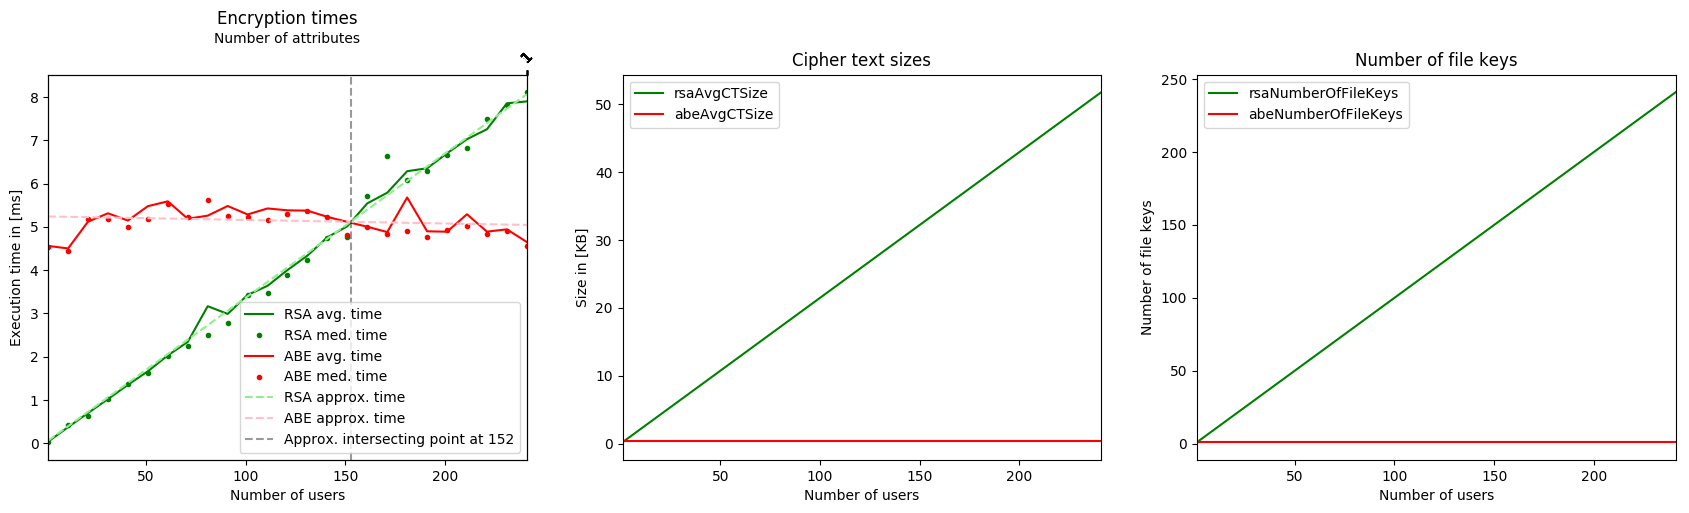
\includegraphics[width=\linewidth]{img/eval-and-policy/encrypt_incrementing_10.png}
    \caption{$1$-for-$\infty$ configuration using "and"-policy}
    \label{fig:1-for-infty-and}
\end{figure}
\begin{figure}[!t]
\centering
    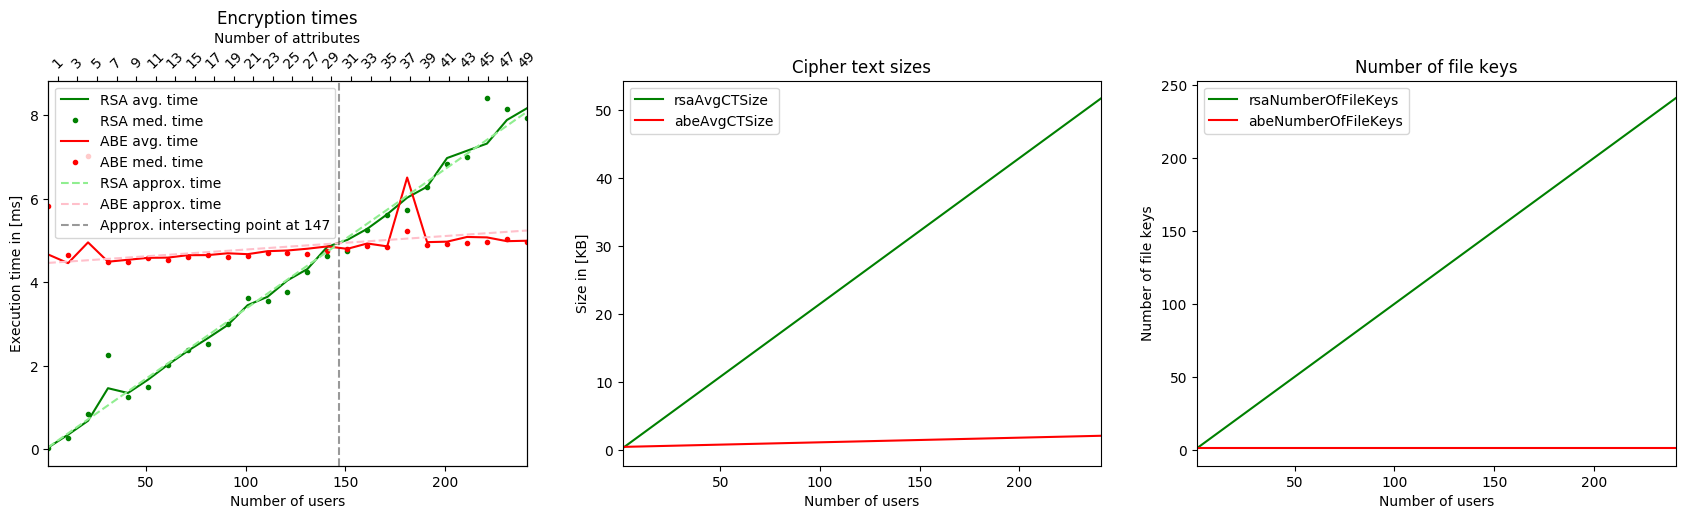
\includegraphics[width=\linewidth]{img/eval-and-policy/encrypt_incrementing_10_attribute_increment_1per5User.png}
    \caption{$1$-for-$5$ configuration using "and"-policy}
    \label{fig:1-for-5-and}
\end{figure}
\begin{figure}[!t]
\centering
    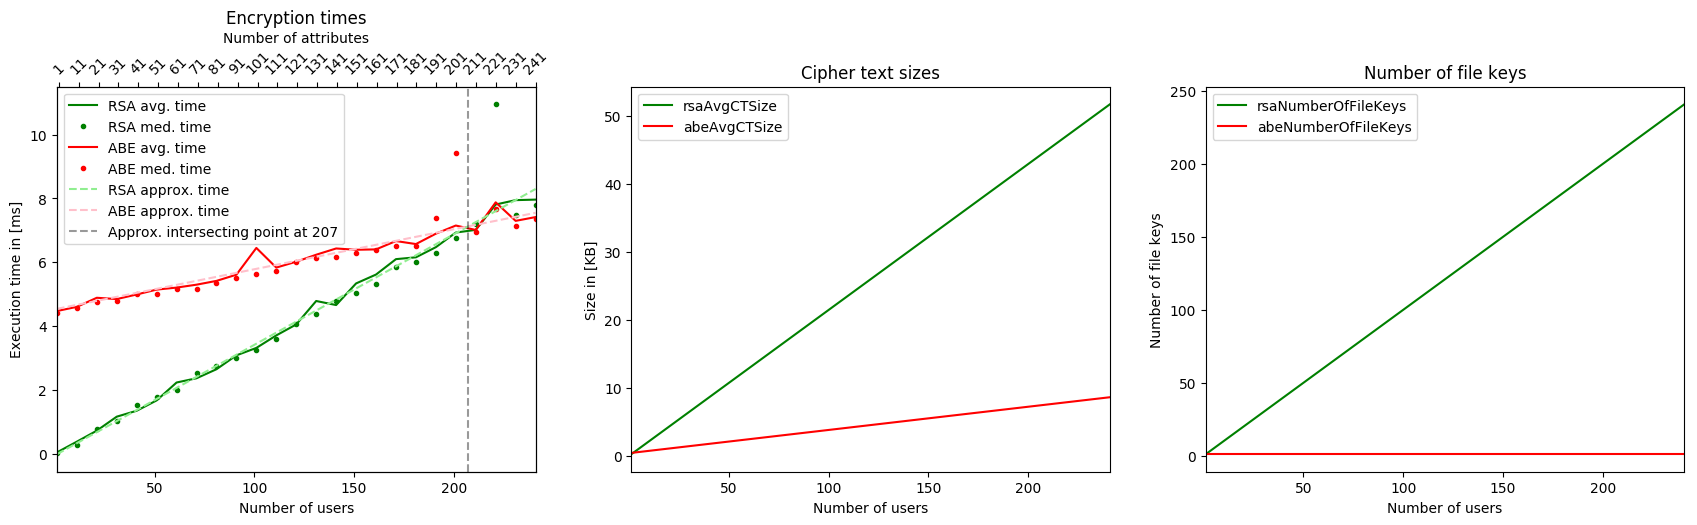
\includegraphics[width=\linewidth]{img/eval-and-policy/encrypt_incrementing_10_attribute_increment_1per1User.png}
    \caption{$1$-for-$1$ configuration using "and"-policy}
    \label{fig:1-for-1-and}
\end{figure}

The configuration of $1$-for-$\infty$ as shown in figure \ref{fig:1-for-infty-and} describes the best-case scenario. Here a group can be complelty described by only one attribute, regardless of the number of users. \name has an constant overhead since the number of attributes remain constant. The intersecting point can be approximated at 145 users. From that point onwards \name scales better then the RSA-based approach. With increasing the number of attributes per user, the overhead of \name becomes greater. In the configuration of $1$-for-$1$, so that each new user introduces a new attribute, the intersecting point gets pushed back to roughly 200 users. 

Comparing the number of file keys over the increasing number of attributes per user, it is obserable that the number of file keys indeed scale truely linearly to the number of users. \name archieves to hold the number of file keys, when using "and"-policies, constant to $1$. The cipher text size raises linearly with increasing number of attributes that need to be embedded into this policy. It still scales better then the RSA based approach. 

\subsubsection{Benchmark: "or"-policies}
\begin{figure}[!t]
\centering
    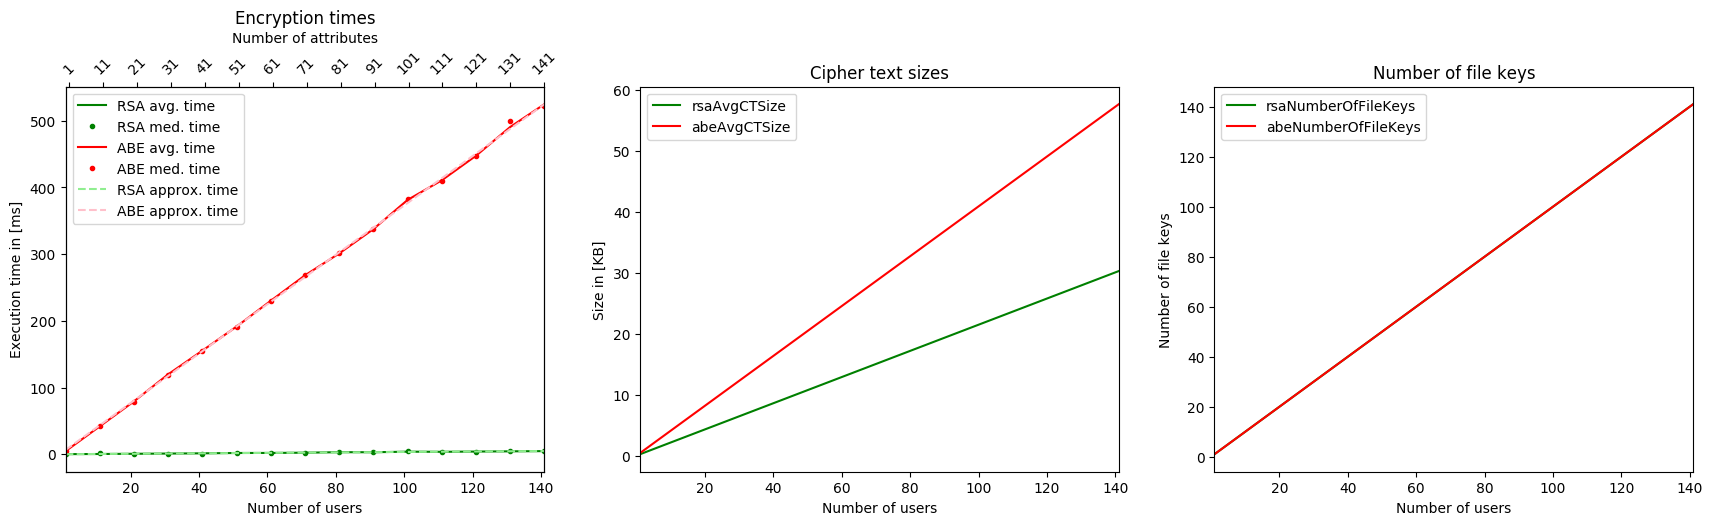
\includegraphics[width=\linewidth]{img/eval-or-policy/encrypt_incrementing_10_attribute_increment_1per1User.png}
    \caption{$1$-for-$1$ configuration using "or"-policy}
    \label{fig:1-for-1-or}
\end{figure}
\begin{figure}[!t]
\centering
    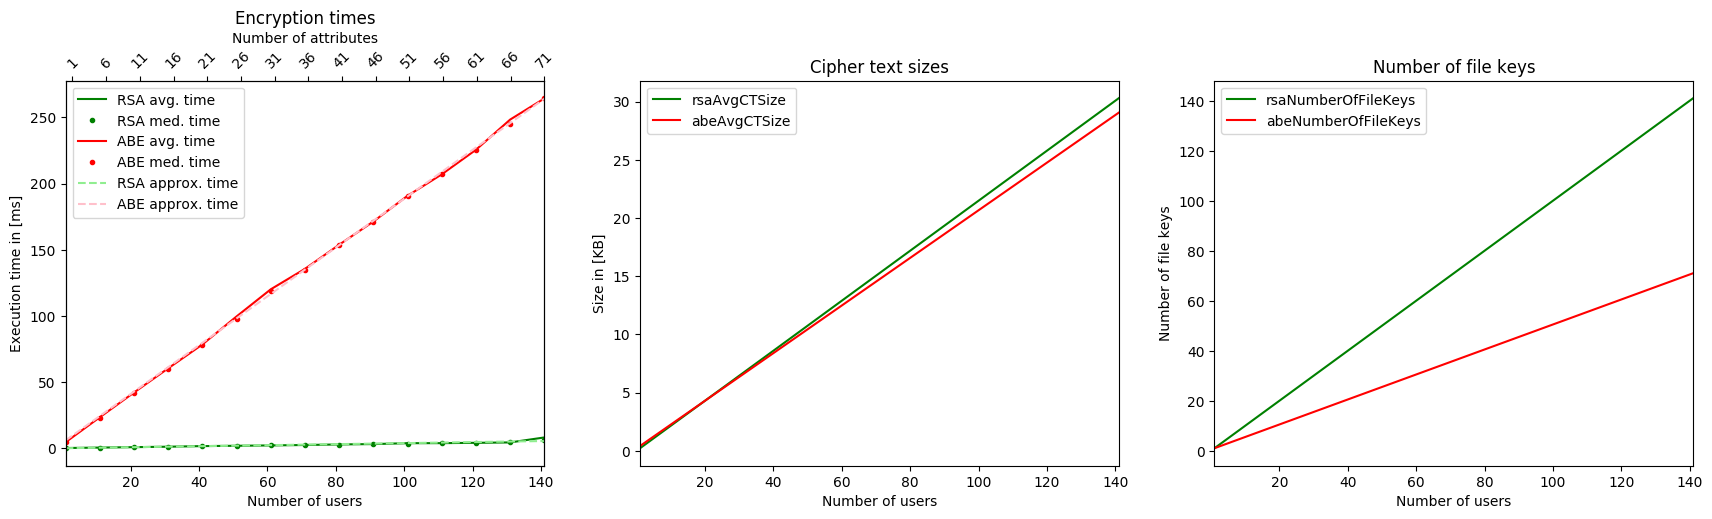
\includegraphics[width=\linewidth]{img/eval-or-policy/encrypt_incrementing_10_attribute_increment_1per2User.png}
    \caption{$1$-for-$2$ configuration using "or"-policy}
    \label{fig:1-for-2-or}
\end{figure}
\begin{figure}[!t]
\centering
    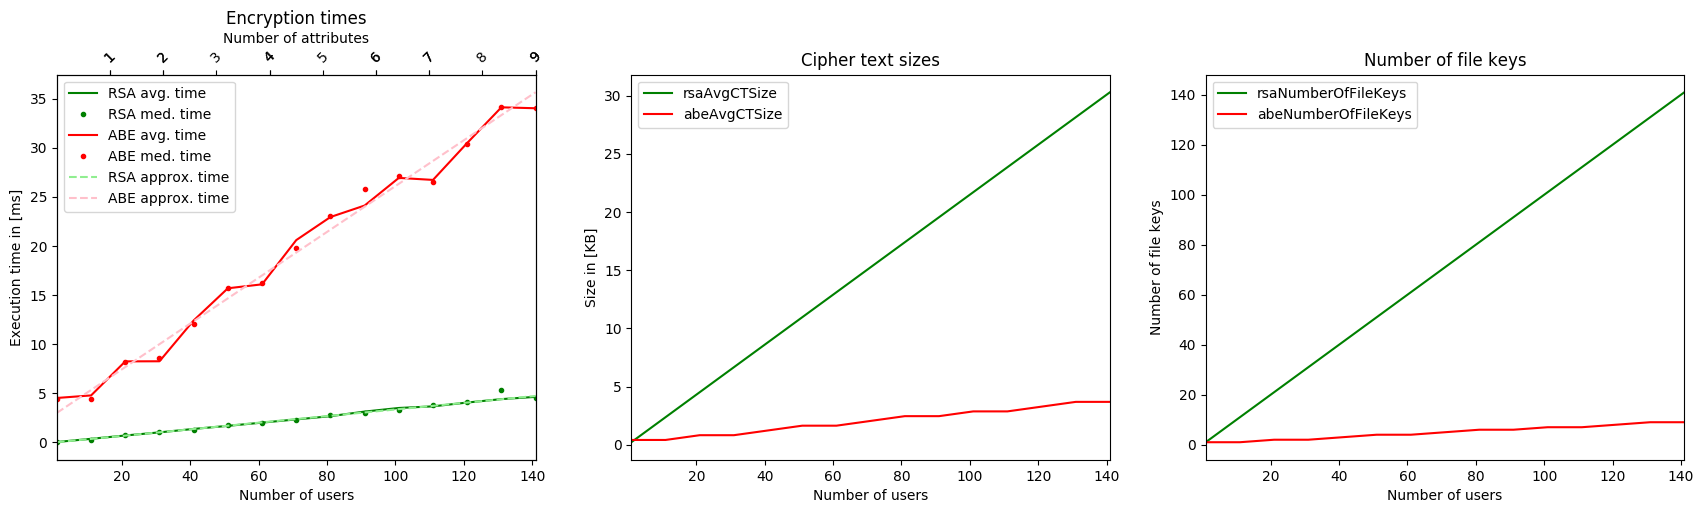
\includegraphics[width=\linewidth]{img/eval-or-policy/encrypt_incrementing_10_attribute_increment_1per16User.png}
    \caption{$1$-for-$16$ configuration using "or"-policy}
    \label{fig:1-for-16-or}
\end{figure}
\begin{figure}[!t]
\centering
    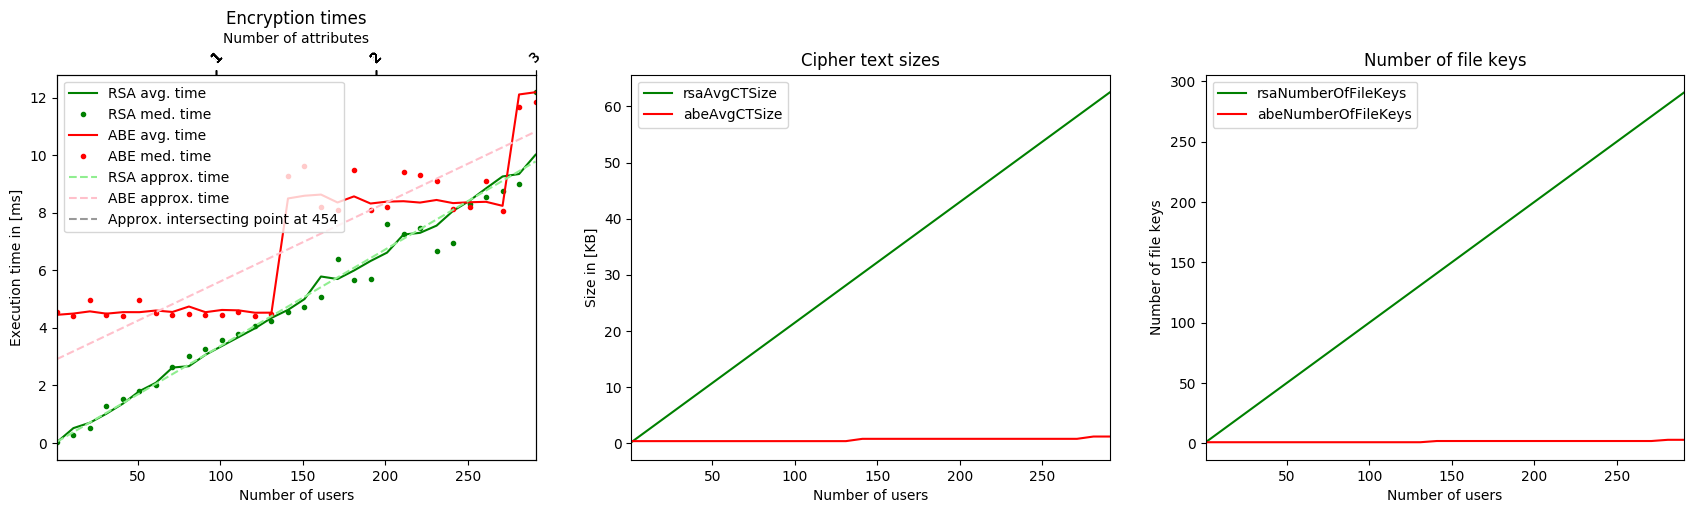
\includegraphics[width=\linewidth]{img/eval-or-policy/encrypt_incrementing_10_attribute_increment_1per140User.png}
    \caption{$1$-for-$140$ configuration using "or"-policy}
    \label{fig:1-for-140-or}
\end{figure}

Complelty different is the benchmark for "or"-policies. Since for each "or" a new cipher text needs to be created \name scales with the number of "or" elements present in the access policy.


%\begin{figure}[!t]
%\centering
%    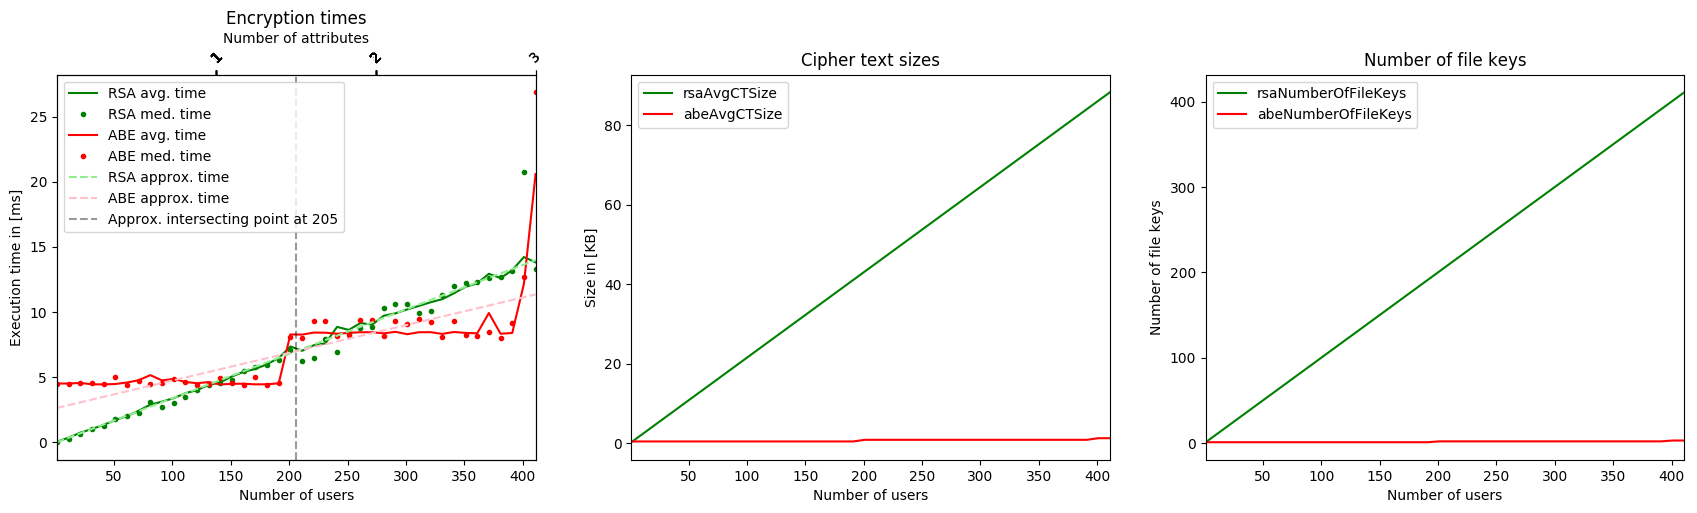
\includegraphics[width=\linewidth]{img/eval-or-policy/encrypt_incrementing_10_attribute_increment_1per200User.png}
%    \caption{$1$-for-$200$ configuration using "or"-policy}
%    \label{fig:1-for-200-or}
%\end{figure}


As it was introduced in the previous chapture, TF-DAC-MACS was adapted to support access policies that are present DNF-fomular. For each additional "or" and its suptree a new chiper text gets created. This is visible in the Figure \ref{fig:1-for-16-or} in the cipher text size and number of file key graphic. Here a stepwise increasing function is notable. Each step is directly correlated to a new attribute that was included into the policy using konjunction.

The worst-case scenario, as introduced in section \ref{sec:upper-bound-and-worst-case-scenario}, is defined as the scenarion were the number of users is equal the number of attributes in an or-policy. This case is shown in figure \ref{fig:1-for-1-or}. In that case is encryption time of \name two magintues higher ($\approx 0-550$ms) than the computation time of the RSA-approach ($\approx 0-10$ms). Even the cipher text size is substantial greater than the cipher text size per file key. This results from the fact that now, \name scales with the same overhead as the RSA approach regarding the number of file keys. So no adventage could be gained over the RSA approach in the worst-case scenario.

Interessting to notice is if a configuration of one attribute per two users is used (Figure \ref{fig:1-for-2-or}) the file keys scale twice as good and the cipher text size scale rather similar to the size of the RSA based file keys. 

Reducing the overhead to a 1-for-16 configuration using "or"-policies, as shown in Figure \ref{fig:1-for-16-or}, a step wise function is notable in each of the plottet functions. The next step happens each 16 users - each attribute. The less attributes are used to describe a user group using "or"-policies, the better does \name scale. Since the number of attributes and the number of cipher text are directly correltated, a great adventage over the classical RSA-based appraoch can be archieved.

Finally, in Figure \ref{fig:1-for-140-or}, a configuration was when \name can b expected to scale better then the RSA-based appraoch. When a group of user can be described by a policy that utalized no "or" for at least 140 members, the assumption can be made that \name scales better regarding computation time in comparison to the classical RSA-based appraoch. 

In general it holds true that the regarding the cipher text size and the number of file keys \name scales better if a group of user can be described by "or" conditions then there are users. 

\subsection{Member Join}
On member join, in RSA each file key needs to be reencrypted for the new member. Using the ABE appraoch simply a attribute key that matches the group policy needs to be created. 

\subsubsection{Assumption}
Given the previous statement, it can be assumped that \name scales with an constant overhead and the RSA approach scales linearly with the increasing number of cipher texts.

\subsubsection{Benchmark: Member Join}
\begin{figure}[!ht]
\centering
    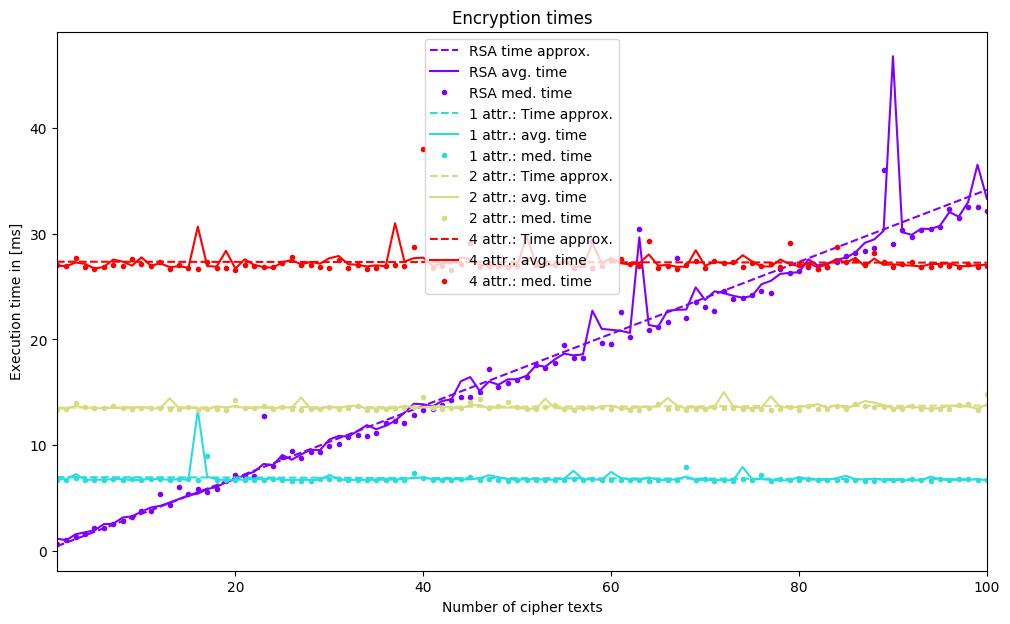
\includegraphics[width=\linewidth]{img/eval-join/join_attr_1.png}
    \caption{Rekeying for one new member. Scaled over the number of attributes}
    \label{fig:member-join}
\end{figure}

As shown in figure \ref{fig:member-join} the assumption can be supported. Three group configurations were evaluated. Having 1, 2 or 4 attributes respectivcally. Depending on the number of attributes the intersecting points of 20, 40 and 90 cipher texts can be extracted. After this amount of attributes \name is faster in adding members to a group. 

\subsection{Member Leave}
Member Leave comes with a greater overhead for \name. Additionally all cipher text need to be updated, each non-revoker user need to revieve a new update key, and the cipher text update key, user secret update key and new attribute value private and public key need to be calculated. On the other hand is the biggest adventage of the RSA-based appraoch that simply the respective file keys of the revoked user need to be deleted.

\subsubsection{Assumption}
The assumption is simply stated that \name can not scale better then the RSA-based approach. Even the attribute value key creation might take longer then just removing the saved file keys for the respektive user. 

\subsubsection{Benchmark: Member Leave}
\begin{figure}[!ht]
\centering
    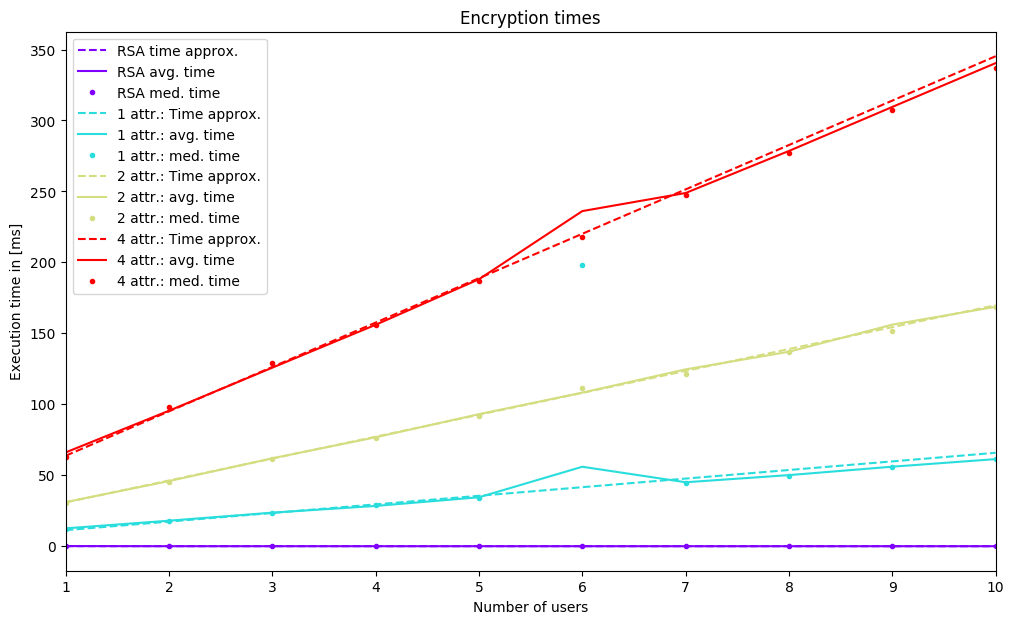
\includegraphics[width=\linewidth]{img/eval-leave/leave_attr_1_users_2.png}
    \caption{One member leaves the share. Scaled over the number of attributes}
    \label{fig:member-leave}
\end{figure}

Figure \ref{fig:member-leave} shows the exact expected behavior. For already one cipher text the gab between the different number of attributes and the RSA-based approach is crealy notable. More attributes means here that a user was revoked that owned multible attribute, which each need to be revoked by itself. 

In a real world system the cipher text update and the user secret key update would happen on the server and client device side. Further it could also happen in parallel to speed up this process. Still it holds true, that \name scales definilty much worse then the RSA-based approach.


% Conclusion
\chapter{Conclusion}
In this thesis a solution to the scalability problem of classical RSA-based group sharing scheme was given with respect to not violate any security requirements \ref{sec:requirements} that where already present in the reference system. Classical systems suffer from many file-keys that need to be maintained each time a new file is updated or a new member joins a group. Existing members need to make sure that the newly joined member can access all previous shared files by decrypting all file-keys and encrypting them again with the new members public key, creating own file keys for the new member. If a new file is updated, it need to made accessable to all members in the group. A file need to be encrypted one by one for each public key in the group. Creating $n$ more file-keys per file upload.

Different approaches are analyzed and argumentatively compared to end-up with an MA-ABE scheme fits the requirements and solves the scalability problem the best.  MA-ABE uses attribute to create an access policy under which a file is secured. This access policy acts like a shared group key that is only accessible to the members that satisfy this access policy. In that way does MA-ABE solves the initial problem of creating $n$ file keys per new file update. Each scheme using a group key only needs to encrypt the file once using the group key resulting in one shared file-key. 

MA-ABE was chosen as the best candidate, because it, in comparison to other secure-group communications, does not redistribute the shared group key to other members. The main feature of an ABE scheme is that the users inherently possesses all needed information to calculate the group key from their given attribute secrets. 

MA-ABE is especially important in the field of applied ABE schemes, since it divides the universe of attributes into different separated clusters, each managed and maintained by an own, self-organized AA. This breaks up a disadvantage of classical ABE schemes: the global decryption power of the system administrator or single AA. 

From the current field of MA-ABE schemes TF-DAC-MACS was the candidate that showed great scalability and performance, no global decryption power of the CA and a mechanism to revoke users from the system. Since it does not support 1-of-n threshold gate policies (OR-gates), an improved version to this scheme, called \name, was constructed and implemented. To further make \name more practically applicable the fix two-factor constrain was made optional. 

To evaluate whether \name indeed scales better than the classical rekeying scheme different benchmarks were performed against a reference implementation of the classical RSA-based rekeying scheme. The outcome was that regarding the number of file-keys \name scales better with a worst-case scenario were \name scales in the same way as the reference implementation. However, it was noticeable that this feature comes with additional overhead in file-key size. Taking this observation into account archives the prototype a better scalability when at most $n/2$ "OR"-gates are used in the access policy. 

Regarding performance a completely different picture is drawn. Due to the assumption that the number of attributes to describe a group is equal or less to the number of users in the group \name shows a better performance since it only works with the attributes and not the users directly. Depending on the underlying system and the chosen distribution of attributes to users an intersecting point can be calculated when \name shows a better performance. This intersecting point is located in the best-case scenario (Figure \ref{fig:1-for-infty-and}) at around 145 users. 

To achieve a better single encryption performance than the classical system at least 145 users need to be describable with one attribute. The resulting implication is that \name benefits from large scale systems with a lot of users that share a lot of attributes. Small groups that share perform peer-to-peer sharing suffer more from the additional overhead. Here \name can only be beneficial if storage and not computing power is the bottleneck. 

\section{Practical Applicability}

\begin{figure}[!ht]
\centering
    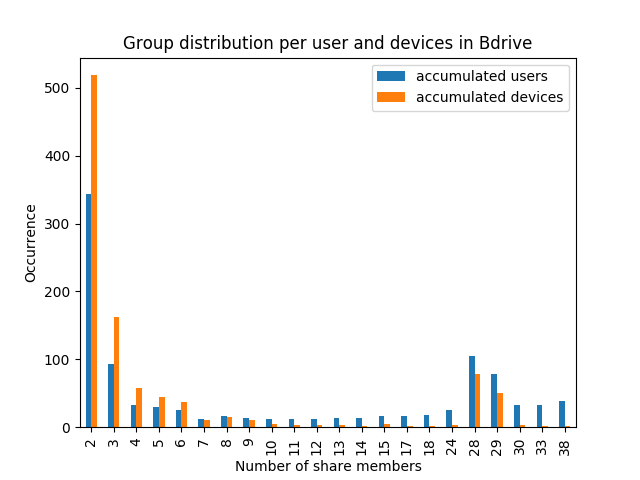
\includegraphics[width=1.0\linewidth]{img/share_distribution_bdirve.png}
    \caption{The distribution of shared folders per users and their aggregated devices.}
    \label{fig:evaluation-share-distribution}
\end{figure}

In the evaluation capture \ref{sec:evaluation} it was concluded that in the best-case scenario \name performs and scales better than the Bdrive from 145 users in a group onwards if they all can be described by the same attribute. To validate that is a common scenario in the real world the distribution of groups and their members of Bdrive are listed in Figure \ref{fig:evaluation-share-distribution}.

As it can be extracted from the figure, many users share file only to one or two other users. In that case would \name provide no performance  advantage. Really interesting for the ABE use case is the second spike at 28 to 30 members. Since Bdrive is addressed to business it can be assumed that this second spike define the company wide shared folders. It can be expected that for very large scale companies that have more then 300 employees. If they all are members in the same share/name can use its full potential, since all members will share a common attribute: "Employee in Company X".

In conclusion \name can reduce the number of file-keys dramatically if combined with the right access policy. It depends on the company administrator to assign each user suitable attributes so that fine-grain access formulas without using "OR"-gates can be constructed.  
\section{Future adaptations}

\todo{
* Data owner Id can relate to the selected two factor key. 
* This would enable us to have multible keys 2FA keys per user. each securing an own CT. 
* make ownerId -> 2FA id 

* Handle attributes on device level and not on user level 
}

%----------------------------------------------------------------------------------------
%	THESIS CONTENT - APPENDICES
%----------------------------------------------------------------------------------------

\appendices % Cue to tell LaTeX that the following "chapters" are Appendices

%----------------------------------------------------------------------------------------
%	BIBLIOGRAPHY
%----------------------------------------------------------------------------------------
\printbibliography[heading=bibintoc]


%----------------------------------------------------------------------------------------

\end{document}  
